% Options for packages loaded elsewhere
\PassOptionsToPackage{unicode}{hyperref}
\PassOptionsToPackage{hyphens}{url}
%
\documentclass[
  10pt,
  twoside,nohyper]{book}
\usepackage{amsmath,amssymb}
\usepackage{iftex}
\ifPDFTeX
  \usepackage[T1]{fontenc}
  \usepackage[utf8]{inputenc}
  \usepackage{textcomp} % provide euro and other symbols
\else % if luatex or xetex
  \usepackage{unicode-math} % this also loads fontspec
  \defaultfontfeatures{Scale=MatchLowercase}
  \defaultfontfeatures[\rmfamily]{Ligatures=TeX,Scale=1}
\fi
\usepackage{lmodern}
\ifPDFTeX\else
  % xetex/luatex font selection
\fi
% Use upquote if available, for straight quotes in verbatim environments
\IfFileExists{upquote.sty}{\usepackage{upquote}}{}
\IfFileExists{microtype.sty}{% use microtype if available
  \usepackage[]{microtype}
  \UseMicrotypeSet[protrusion]{basicmath} % disable protrusion for tt fonts
}{}
\makeatletter
\@ifundefined{KOMAClassName}{% if non-KOMA class
  \IfFileExists{parskip.sty}{%
    \usepackage{parskip}
  }{% else
    \setlength{\parindent}{0pt}
    \setlength{\parskip}{6pt plus 2pt minus 1pt}}
}{% if KOMA class
  \KOMAoptions{parskip=half}}
\makeatother
\usepackage{xcolor}
\usepackage{longtable,booktabs,array}
\usepackage{calc} % for calculating minipage widths
% Correct order of tables after \paragraph or \subparagraph
\usepackage{etoolbox}
\makeatletter
\patchcmd\longtable{\par}{\if@noskipsec\mbox{}\fi\par}{}{}
\makeatother
% Allow footnotes in longtable head/foot
\IfFileExists{footnotehyper.sty}{\usepackage{footnotehyper}}{\usepackage{footnote}}
\makesavenoteenv{longtable}
\usepackage{graphicx}
\makeatletter
\def\maxwidth{\ifdim\Gin@nat@width>\linewidth\linewidth\else\Gin@nat@width\fi}
\def\maxheight{\ifdim\Gin@nat@height>\textheight\textheight\else\Gin@nat@height\fi}
\makeatother
% Scale images if necessary, so that they will not overflow the page
% margins by default, and it is still possible to overwrite the defaults
% using explicit options in \includegraphics[width, height, ...]{}
\setkeys{Gin}{width=\maxwidth,height=\maxheight,keepaspectratio}
% Set default figure placement to htbp
\makeatletter
\def\fps@figure{htbp}
\makeatother
\setlength{\emergencystretch}{3em} % prevent overfull lines
\providecommand{\tightlist}{%
  \setlength{\itemsep}{0pt}\setlength{\parskip}{0pt}}
\setcounter{secnumdepth}{5}
\usepackage{geometry}
\geometry{
  a4paper,
  top=2.5cm,
  bottom=2.5cm,
  inner=3cm,
  outer=3cm
}
\usepackage{pdfpages}


\renewcommand{\baselinestretch}{1.15}
\parskip=6pt

\definecolor{azulUC3M}{RGB}{0,0,102}
\definecolor{gray97}{gray}{.97}
\definecolor{gray75}{gray}{.75}
\definecolor{gray45}{gray}{.45}

\usepackage[a-1b]{pdfx}

\usepackage{hyperref}
\hypersetup{colorlinks=true,
	linkcolor=black, % enlaces a partes del documento (p.e. índice) en color negro
	urlcolor=blue} % enlaces a recursos fuera del documento en azul


\usepackage{amsmath,amssymb,amsfonts,amsthm}

\usepackage{txfonts} 
\usepackage[T1]{fontenc}
\usepackage[utf8]{inputenc}

\usepackage[english]{babel} 
\usepackage[babel, english=american]{csquotes}
\AtBeginEnvironment{quote}{\small}

% diseño de PIE DE PÁGINA
\usepackage{fancyhdr}
\pagestyle{fancy}
\fancyhf{}
\renewcommand{\headrulewidth}{0pt}
\rfoot{\thepage}
\fancypagestyle{plain}{\pagestyle{fancy}}


\usepackage{titlesec}
\usepackage{titletoc}
\titleformat{\chapter}[block]
{\large\bfseries\filcenter}
{\thechapter.}
{5pt}
{\MakeUppercase}
{}
\titlespacing{\chapter}{0pt}{0pt}{*3}
\titlecontents{chapter}
[0pt]                                               
{}
{\contentsmargin{0pt}\thecontentslabel.\enspace\uppercase}
{\contentsmargin{0pt}\uppercase}                        
{\titlerule*[.7pc]{.}\contentspage}                 

\titleformat{\section}
{\bfseries}
{\thesection.}
{5pt}
{}
\titlecontents{section}
[5pt]                                               
{}
{\contentsmargin{0pt}\thecontentslabel.\enspace}
{\contentsmargin{0pt}}
{\titlerule*[.7pc]{.}\contentspage}

\titleformat{\subsection}
{\normalsize\bfseries}
{\thesubsection.}
{5pt}
{}
\titlecontents{subsection}
[10pt]                                               
{}
{\contentsmargin{0pt}                          
	\thecontentslabel.\enspace}
{\contentsmargin{0pt}}                        
{\titlerule*[.7pc]{.}\contentspage}  



\usepackage{multirow} %permite combinar celdas 
\usepackage{caption} %para personalizar el título de tablas y figuras
\usepackage{floatrow} %utilizamos este paquete y sus macros \ttabbox y \ffigbox para alinear los nombres de tablas y figuras de acuerdo con el estilo definido. Para su uso ver archivo de ejemplo 
\usepackage{array} % con este paquete podemos definir en la siguiente línea un nuevo tipo de columna para tablas: ancho personalizado y contenido centrado
\newcolumntype{P}[1]{>{\centering\arraybackslash}p{#1}}
\DeclareCaptionFormat{upper}{#1#2\uppercase{#3}\par}


% Diseño de tabla para ingeniería
\captionsetup[table]{
	format=upper,
	justification=centering,
	labelsep=period,
	width=.75\linewidth,
	labelfont=small,
	font=small,
}




\usepackage{graphicx}
\graphicspath{{imagenes/}} %ruta a la carpeta de imágenes

% Diseño de figuras para ingeniería
\captionsetup[figure]{
	format=hang,
	name=Fig.,
	singlelinecheck=off,
	labelsep=period,
	labelfont=small,
	font=small		
}




\usepackage{chngcntr}
\counterwithout{footnote}{chapter}


\usepackage{listings}


\lstdefinestyle{estilo}{ frame=Ltb,
	framerule=0pt,
	aboveskip=0.5cm,
	framextopmargin=3pt,
	framexbottommargin=3pt,
	framexleftmargin=0.4cm,
	framesep=0pt,
	rulesep=.4pt,
	backgroundcolor=\color{gray97},
	rulesepcolor=\color{black},
	%
	basicstyle=\ttfamily\footnotesize,
	keywordstyle=\bfseries,
	stringstyle=\ttfamily,
	showstringspaces = false,
	commentstyle=\color{gray45},     
	%
	numbers=left,
	numbersep=15pt,
	numberstyle=\tiny,
	numberfirstline = false,
	breaklines=true,
	xleftmargin=\parindent
}

\captionsetup[lstlisting]{font=small, labelsep=period}

\lstset{style=estilo}
\renewcommand{\lstlistingname}{\uppercase{Código}}

% Define the color azulUC3M
\definecolor{azulUC3M}{RGB}{0,0,102}

% Redefine \maketitle
\makeatletter
\renewcommand{\maketitle}{%
	\begin{titlepage}
		\begin{sffamily}
			\color{azulUC3M}
			\begin{center}
				
\includegraphics[width=16cm]{imagenes/Portada_Logo.png}\\[1cm]
				\begin{Large}
					Master Degree in...\\			
					Academic Year (e.g., 2018-2019)\\
					\vspace{1cm}		
					\textsl{Master Thesis}\\
					\bigskip
				\end{Large}
				{\Huge  Introducing Offside Control: a Football Analytics Parameter to Evaluate Offside Performance}\\
				\vspace*{0.5cm}
				\rule{10.5cm}{0.1mm}\\
				\vspace*{0.9cm}
				{\LARGE Alvaro Novillo Correas}\\ 
				\vspace*{1cm}
				\begin{Large}
					1st Tutor complete name\\
					2nd Tutor complete name\\
					Place and date\\
				\end{Large}
			\end{center}

			\vfill
			\color{black}
			\begin{footnotesize}
				\noindent\fbox{
					\begin{minipage}{\textwidth}
						\textbf{AVOID PLAGIARISM}\\
						The University uses the \textbf{Turnitin Feedback Studio} program within the Aula Global for the delivery of student work. This program compares the originality of the work delivered by each student with millions of electronic resources and detects those parts of the text that are copied and pasted. Plagiarizing in a TFM is considered a \textbf{Serious Misconduct}, and may result in permanent expulsion from the University.
					\end{minipage}	
				}
				\vspace*{.5cm}\\	
				\noindent
\includegraphics[width=4.2cm]{imagenes/creativecommons.png}\\
				\emph{[Include this code in case you want your Master Thesis published in Open Access University Repository]}\\
				This work is licensed under Creative Commons \textbf{Attribution – Non Commercial – Non Derivatives}
			\end{footnotesize}
		\end{sffamily}
	\end{titlepage}
}
\makeatother


\usepackage{booktabs}
\usepackage{longtable}
\usepackage{array}
\usepackage{multirow}
\usepackage{wrapfig}
\usepackage{float}
\usepackage{colortbl}
\usepackage{pdflscape}
\usepackage{tabu}
\usepackage{threeparttable}
\usepackage{threeparttablex}
\usepackage[normalem]{ulem}
\usepackage{makecell}
\usepackage{xcolor}
\ifLuaTeX
  \usepackage{selnolig}  % disable illegal ligatures
\fi
\usepackage[]{natbib}
\bibliographystyle{abbrvnat}
\usepackage{bookmark}
\IfFileExists{xurl.sty}{\usepackage{xurl}}{} % add URL line breaks if available
\urlstyle{same}
\hypersetup{
  pdftitle={Introducing Offside Control: a Football Analytics Parameter to Evaluate Offside Performance},
  pdfauthor={Álvaro Novillo Correas},
  hidelinks,
  pdfcreator={LaTeX via pandoc}}

\title{Introducing Offside Control: a Football Analytics Parameter to Evaluate Offside Performance}
\author{Álvaro Novillo Correas}
\date{2024-03-27}

\begin{document}
\maketitle

{
\setcounter{tocdepth}{1}
\tableofcontents
}
\chapter*{Abstract}\label{abstract}
\addcontentsline{toc}{chapter}{Abstract}

The master thesis explores the application of data analytics in football, with a focus on enhancing understanding and performance through a data driven approach. The study reviews the history and evolution of data analytics in sports, particularly football, and introduces a new methodology for quantifying the effectiveness of offside strategies using Pitch Control models, \emph{Offside Control}. We analize 1,251,934 frames from 100 matches to characterize the Offside Control of 442 players. The methodology combines physical metrics and tactical models derived from tracking datasets, offering insights into the tactical nuances of successful offside strategies. The project's data processing and modeling are conducted using Python, with the source code available in a GitHub repository\footnote{All the source code is inside the code folder at \url{https://github.com/AlvaroNovillo/master_thesis.git}}.

\chapter*{Dedication}\label{dedication}
\addcontentsline{toc}{chapter}{Dedication}

\begin{flushright}
\includegraphics[width=0.17\linewidth,]{imagenes/sign} \end{flushright}

\hfill Álvaro Novillo

\hfill Madrid, May 2024.

\listoffigures
\listoftables

\chapter{Introduction}\label{introduction}

The digital revolution is currently one of the most significant
challenges of our time, altering numerous aspects of society. Football,
in particular, has also been influenced by this transformation.
Technological advancements and digitalization have resulted in a swift
upsurge in the number of measuring devices, data collection and volumes
of data. The leading data companies worldwide, including IBM, Intel, SAP
and Microsoft, are vying for superior data analytics tools and
leveraging sports as an example domain to showcase their products and
brand power \citep{1}.

The practice of data analytics in football has a long history, dating
back to the post-World War II era, when data collection and analysis was
undertaken manually using pencil and paper \citep{1}. It wasn't until
Moneyball was published in 2003 that significant progress began to
emerge: The book, "The Art of Winning an Unfair Game" introduced
sports analytics to a broader audience. It illustrated the use of data
analytics in identifying undervalued players and constructing a
successful team. Since then, data analytics has become an integral
component of sport, football inclusive \citep{1}.

One of the best examples of data analytics being applied to sports is
basketball. Teams use data to analyze player performance, identify
strengths and weaknesses, and develop strategies to win games \citep{2}. They
use in-memory analytics, visualization, the cloud, mobility, camera
footage, and sensors to transform their game. This performance analyses
are of vital importance to a team, aiming to reduce expenditure, enhance
team worth and refine processes across all levels and segments of
operations. The German Football Association (DFB) and the National
Basketball Association (NBA) are two unique cases of digital
transformation from the sports world. Successful teams turn player
performance data into action and gain a competitive advantage.

Over the last years, football analytics has gained significant
popularity, aiming to delve deeper into the game by utilizing advanced
data analysis techniques to optimize team and player performance.

The main objective of this master's thesis is to enhance understanding and performance in football through the use of Data Analytics. The master's thesis includes a literature review of the field, alongside the commonly found data types within this
industry and the main metrics used to analyse player and team performance, focusing on tracking data and Pitch Control models \citep{Spearman}. Following the initial review of the field's state of the art, we propose a new methodology for quantifying the effectiveness of the offside strategy of teams and players using Pitch Control models. Our study defines a new performance parameter, called \emph{Offside Control}, which quantifies the amount of threat posed by the attacking team or player beyond the offside line.

In the study, we will compute both effective and ineffective Offside Control at a rate of 2 frames per second for 100 matches from LaLiga 2019-2020, resulting in a total of 1,251,934 frames analysed. This will allow us to characterize successfully the Offside Control of 442 players in total.

Our proposed methodology aims to contribute to this growing body of knowledge. Analyzing vast amounts of tracking data from LaLiga matches, we seek to uncover patterns in player and team behavior, shedding light on the tactical nuances that underlie successful offside strategies.

All data processing and modeling in this project has been made using python. You can find the source code of the project inside the GitHub repository\footnote{All the source code is inside the code folder at \url{https://github.com/AlvaroNovillo/master_thesis.git}}

\chapter{Data Analytics in football}\label{data-analytics-in-football}

When discussing sports analytics in football, the first metric that
often springs to mind is the Expected Goals (xG) ratio. This statistical
indicator is a predictive Machine Learning (ML) model used to assess the
likelihood of scoring for every shot made in the game. In the context of
each shot, the xG model computes the scoring probability, leveraging a
set of event parameters.

Wyscout xG model, for example, encompass the shot's spatial coordinates,
the assisting player's position, the striking player's use of foot or
head, the type of assist involved, the occurrence of a dribble by either
a field player or the goalkeeper immediately preceding the shot, whether
the shot arises from a set piece, whether it transpires during a
counterattack or in a transitional phase of play, and the subjective
assessment of shot danger as determined by a designated tagger. The
amalgamation of these parameters serves as the foundation for training
the xG model using historical Wyscout data, culminating in the
prediction of the likelihood of a given shot resulting in a goal
\citep{wyscout}.

The probabilities range from 0 to 1. Thus, a shot with an xG value of
0.1 has a 10\% chance of being scored. Penalties have a fixed xG value of
0.76.

Fig. \ref{fig:xg} provides a visual representation of the cumulative development of expected goals
(xG) during the Eibar - Malaga match, which took place on January 15th,
2023 in Spain's second division. Each data point on the graph
corresponds to a shot made by both teams over the course of the game,
offering a comprehensive overview of the evolving scoring opportunities
and outcomes throughout the duration of the game.

\begin{figure}[H]

{\centering 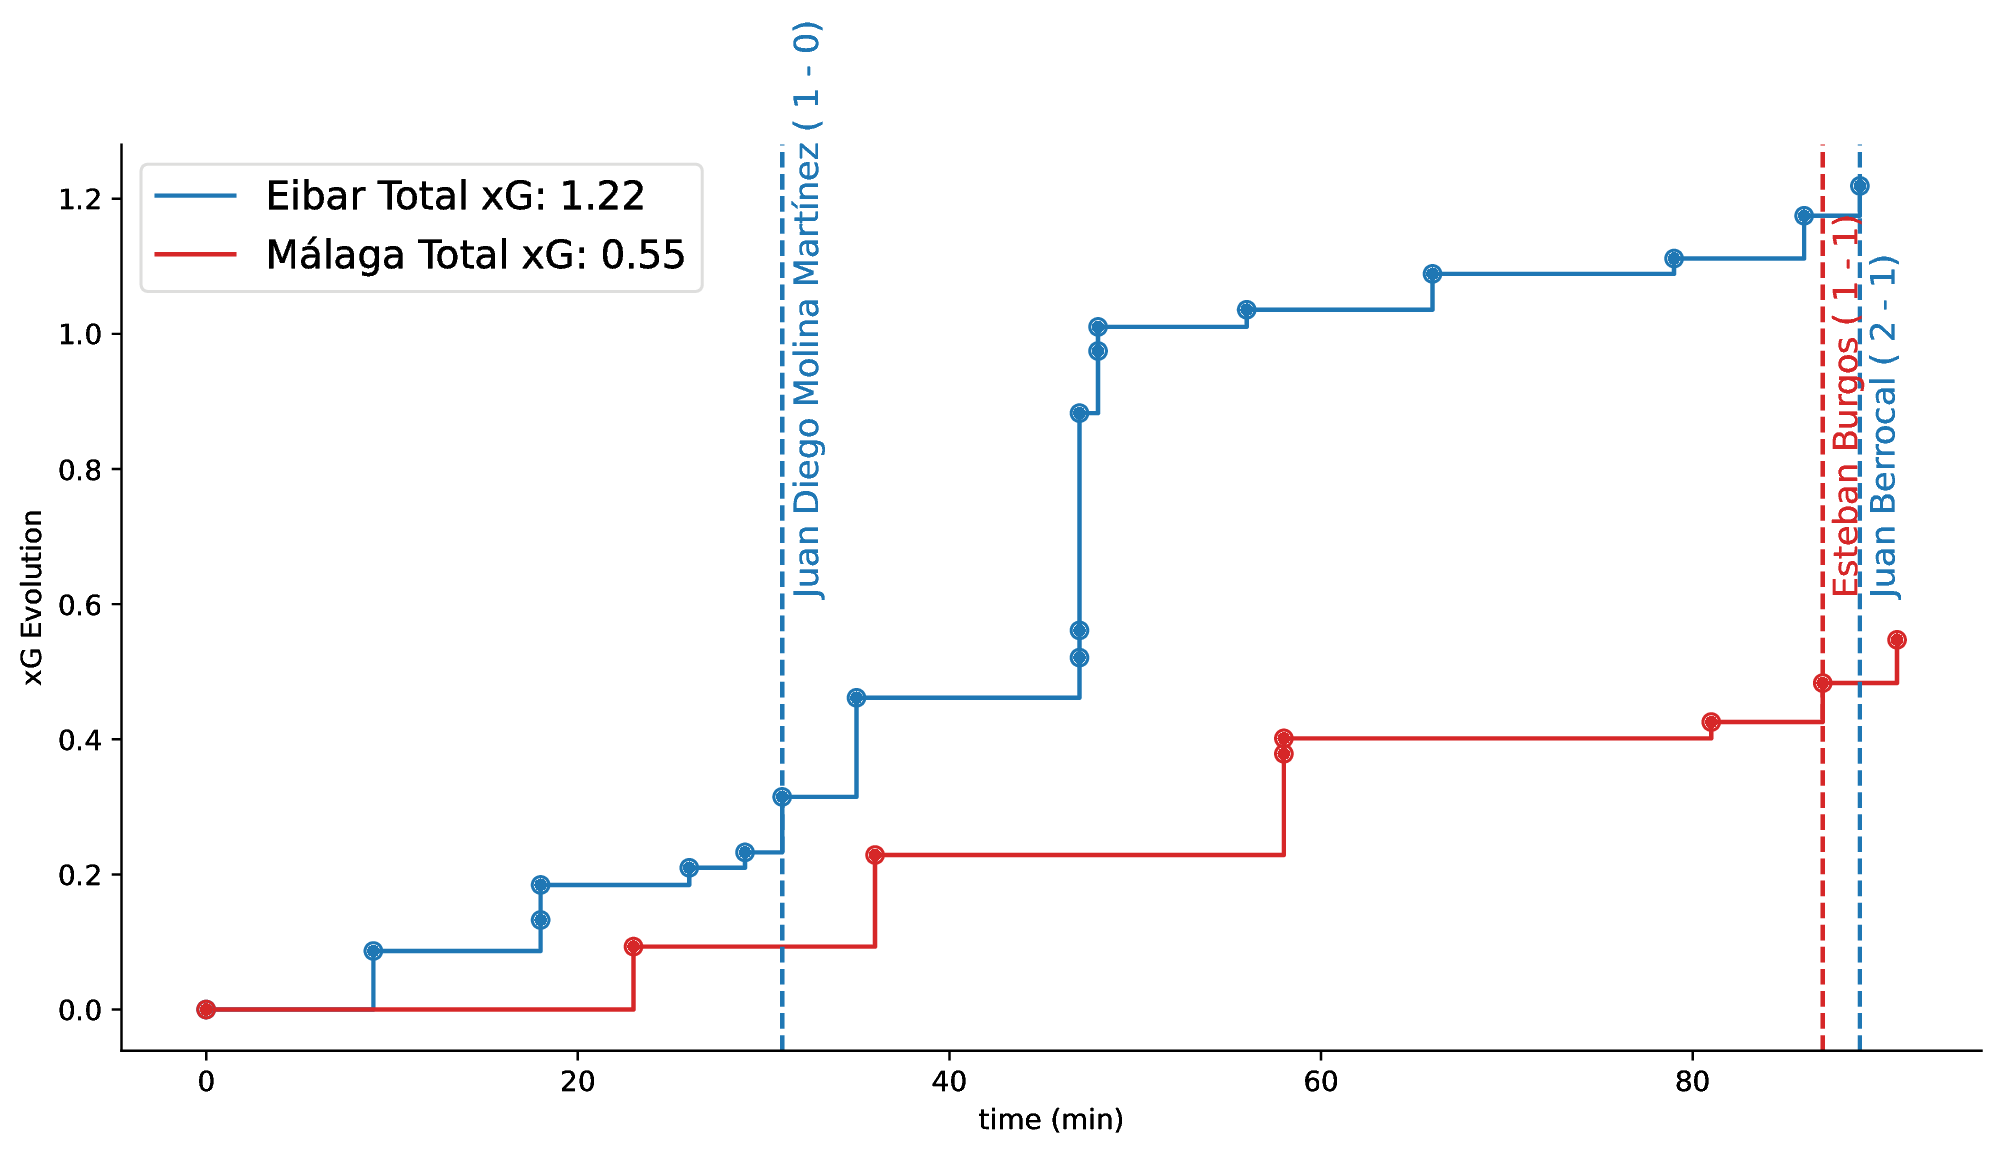
\includegraphics[width=0.8\linewidth,]{imagenes/xg_evol} 

}

\caption{Cumulative development of expected goals (xG) during the Eibar-Malaga match, held on January 15th in Spain’s second division. Each point denotes a shot made by both teams throughout the game. Vertical dashed lines indicate the goal scored, displaying the player and the corresponding score at that specific moment of the match.}\label{fig:xg}
\end{figure}

Expected Goals (xG) have revolutionized the analysis of football by quantifying the quality of scoring opportunities. However, it is important to consider other variables such as player positioning, velocity, passing accuracy, defensive pressure, and tactical formations to gain a broader understanding of the sport. Using the game presented earlier as an example, the next chapter will introduce the broad field of football analytics.

Looking at an xG evolution figure, such as Fig. \ref{fig:xg}, and solely focusing on shot probabilities while disregarding the spatial distribution of shots and occasions feels like merely scratching the surface of what sport analytics can offer to football.

To illustrate the spatial distribution of shot locations taken by both teams during the game, we can create a shot map for each shot. In Fig. \ref{fig:shotmap}, the size of each data point corresponds to the expected goals (xG) generated for the respective shots, providing insights into the perceived scoring potential. Goals scored are visually highlighted with straight lines, indicating the trajectory the ball followed as it found its way into the opponent's net. Bellow each shot map, a plot of the net can be also found, where goals are represented by football balls, and blocked shots by shadowed points. This detailed analysis not only enhances our understanding of scoring opportunities but also sheds light on the tactical strategies employed by both teams, player positioning, and defensive vulnerabilities. Analyses such as the one above are carried out using the most common
source of data in football: \textbf{Events} datasets.

\begin{figure}[H]

{\centering 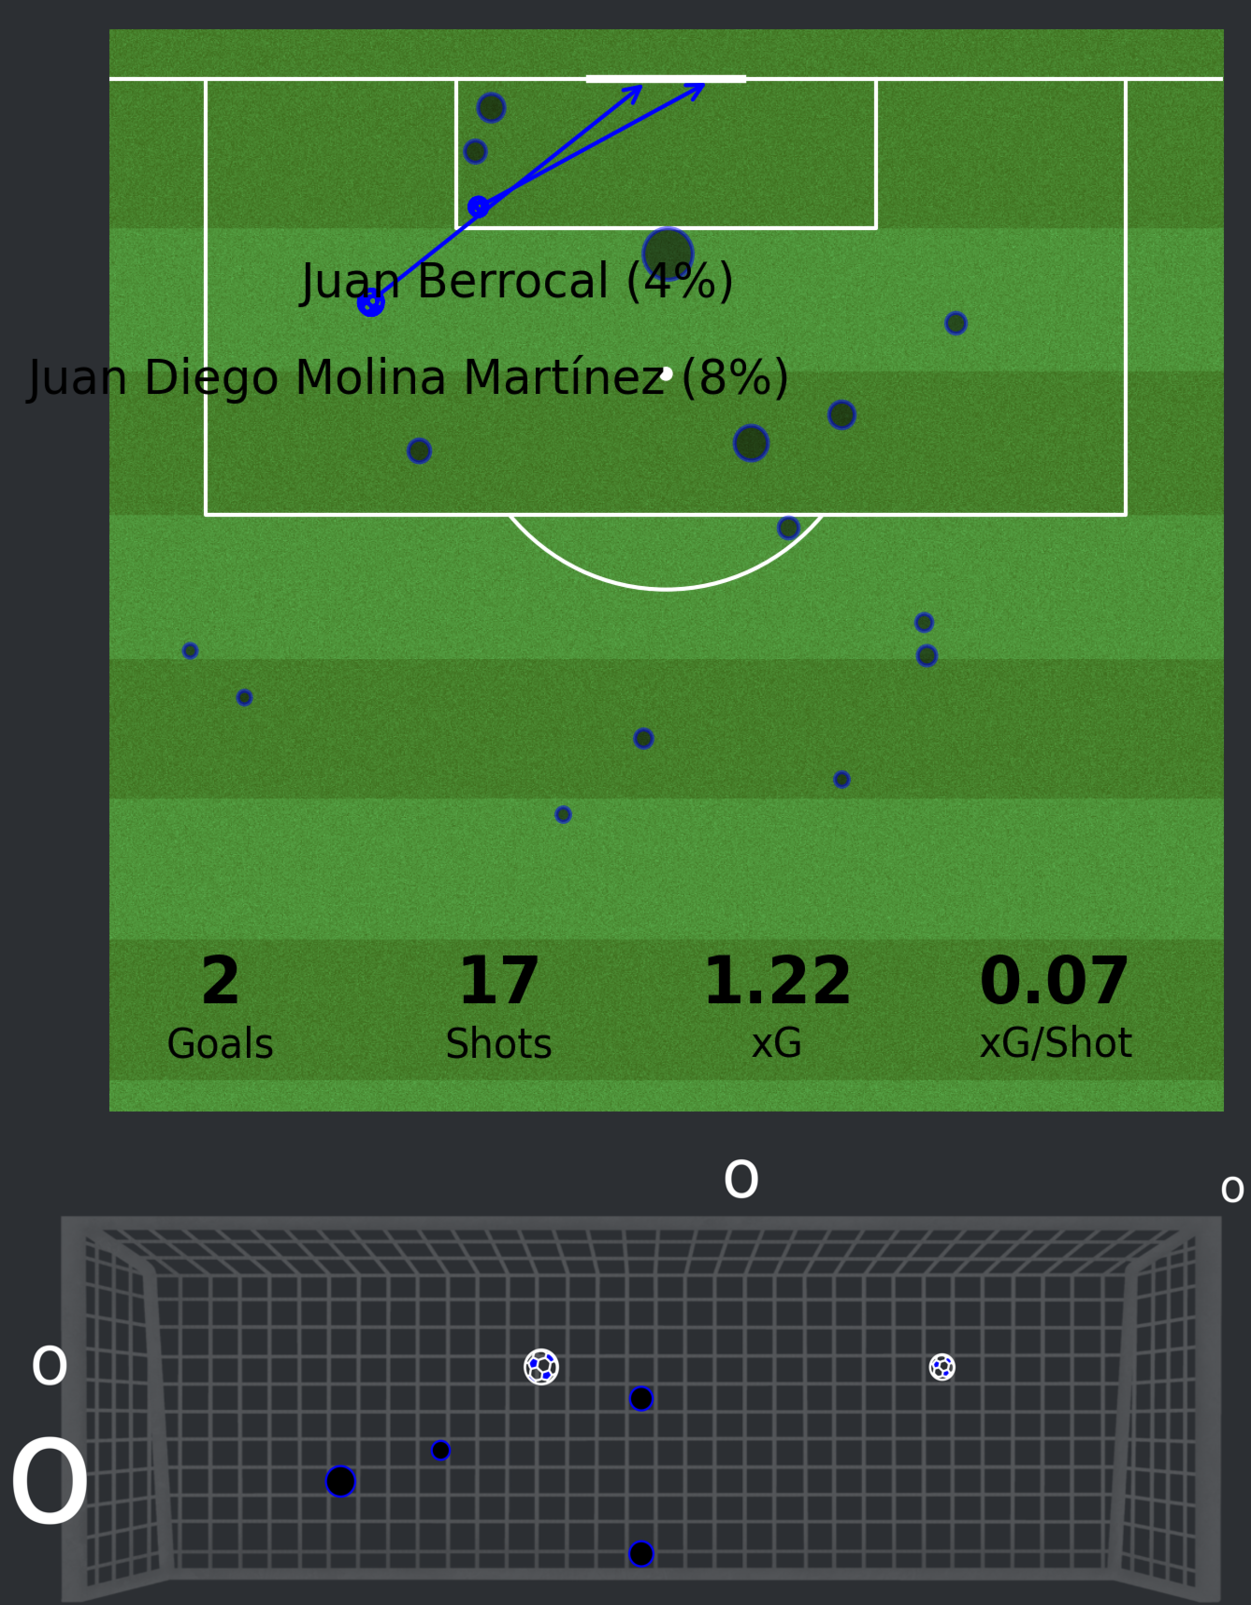
\includegraphics[width=0.45\linewidth,]{imagenes/home_shot_map} 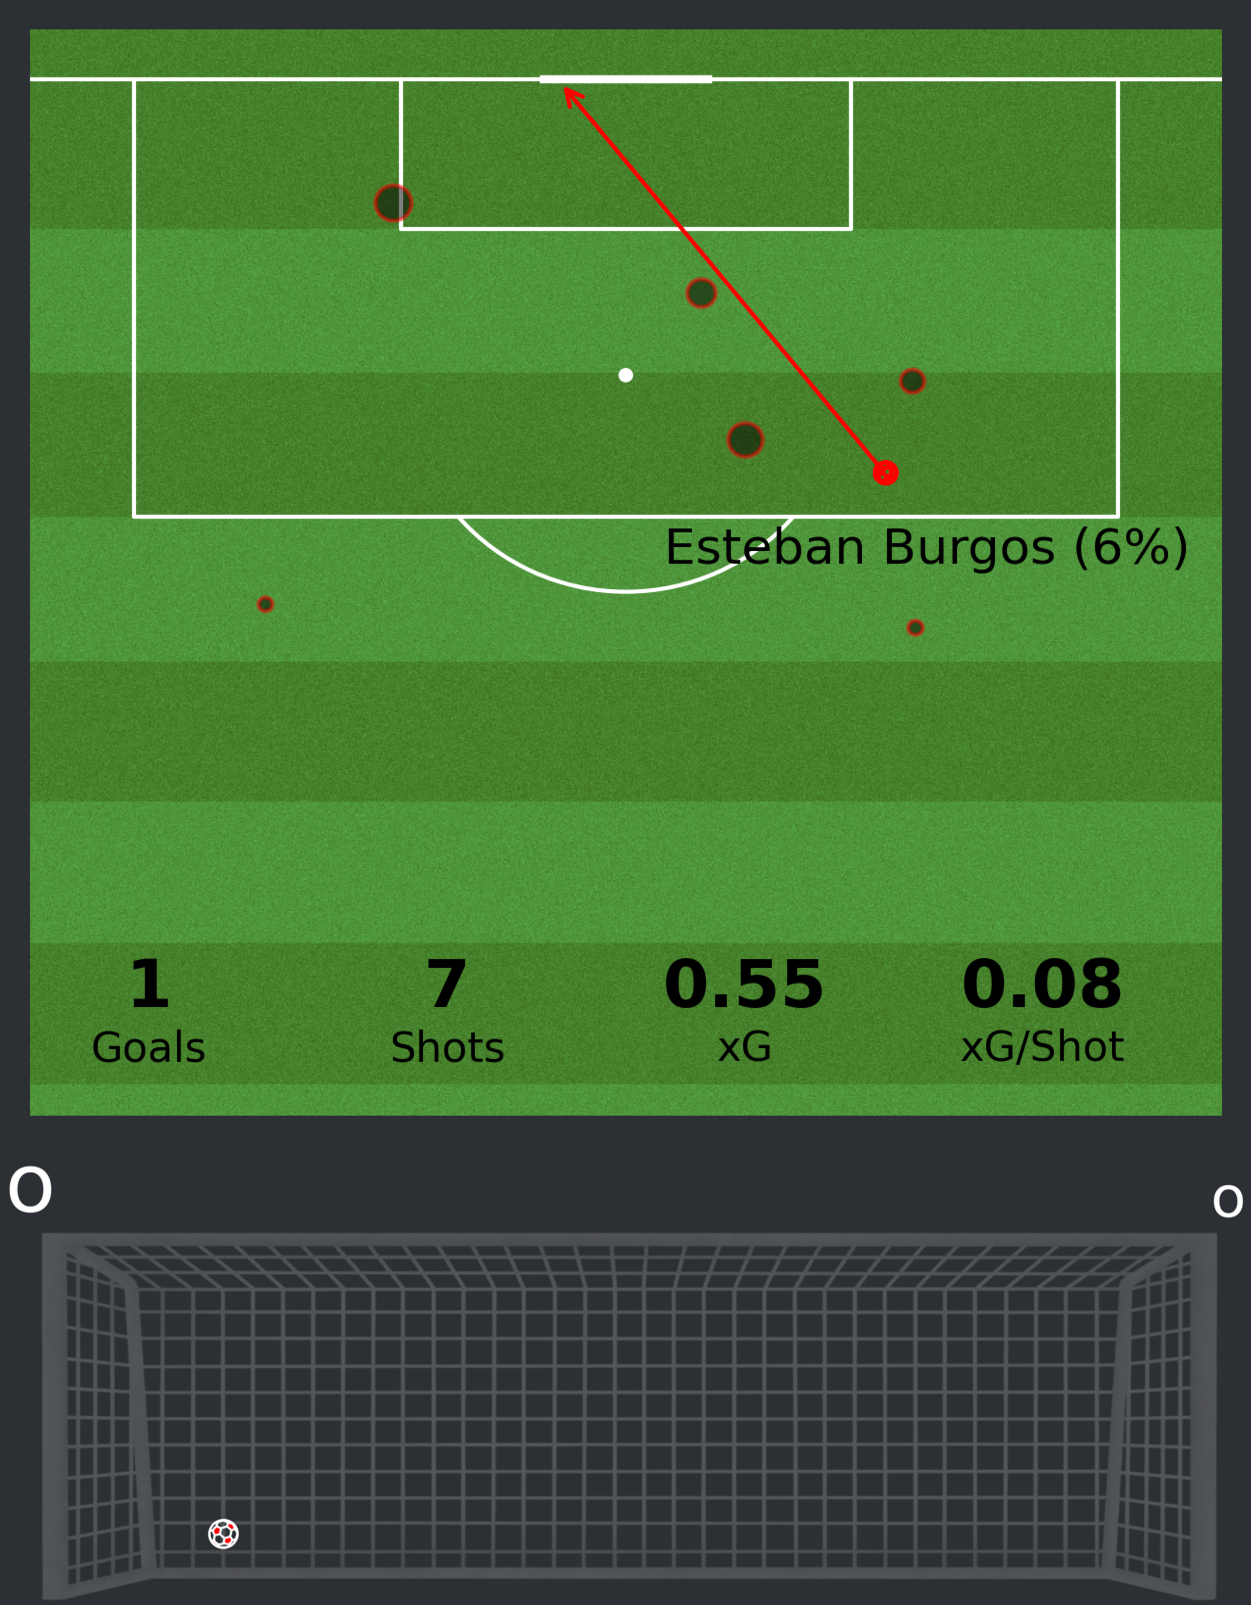
\includegraphics[width=0.45\linewidth,]{imagenes/away_shot_map} 

}

\caption{Shot map of the Eibar (blue, left) - Malaga (red, right) football match. The locations of the points indicate where shots were taken. The size of each point is proportional to the expected goals (xG) generated. Shots that resulted in goals are depicted with a straight line, representing the path the ball took to enter the opponent’s net.}\label{fig:shotmap}
\end{figure}

\section{Events data}\label{events-data}

\texttt{Event\ data} describes specific, human-defined events during a match,
including passes, shots, and fouls. It is captured by human annotators
from various providers. However, this manual process is time-consuming
and typically requires three individuals:

The data collection process is carried out by professional video
analysts (known as operators), who are specialists in football data
collection, using proprietary software (the tagger). The tagger has
undergone several years of development and improvement and is regularly
updated to ensure the highest level of performance is achieved. To
ensure accurate data collection when tagging events in soccer matches,
three operators are assigned: one per team and one supervising the
output of the entire match. This process is based on analysis of the
tagger and soccer match videos. When near-live data delivery is
necessary, a team of four operators may be utilized, with one operator
dedicated to hastening the collection of complex events that require
additional, specific attributes or a quick review \citep{3}.

\begin{table}[!h]
\centering
\caption{\label{tab:event}Example of an events dataset of a game.}
\centering
\resizebox{\ifdim\width>\linewidth\linewidth\else\width\fi}{!}{
\begin{tabular}[t]{rrlrrrrrr}
\toprule
team\_id & code & type & player & x & y & min & sec & period\\
\midrule
174 & 44 & 0aerial\_duel\_lost & 18498 & 71.2 & 25.5 & 0 & 7 & 1\\
174 & 5 & 0ball\_out & 18498 & 77.0 & -1.7 & 0 & 12 & 1\\
178 & 5 & 0ball\_out & 171101 & 70.0 & -1.2 & 0 & 45 & 1\\
178 & 12 & 0despeje\_clearance & 52356 & 29.5 & 85.1 & 1 & 6 & 1\\
178 & 5 & 0ball\_out & 52356 & 25.2 & 101.3 & 1 & 7 & 1\\
\addlinespace
174 & 44 & 0aerial\_duel\_lost & 18498 & 64.2 & 42.4 & 1 & 27 & 1\\
\bottomrule
\end{tabular}}
\end{table}

This type of data structure can be used in a number of ways: it can be
used to measure team performance through general statistics extracted
from event datasets, such as goals, fouls, xG, etc. It can also be used
to create advanced analysis of the team using ensembles of mathematical
tools.

The analysis of the match is furthered through the use of graph theory,
\citep{Buldu}, \citep{NOVILLO2024114355}. Combining
different elements of the events dataset, we can create a graph
corresponding to the passing network of each team, allowing us to
understand the passing structure of both teams.

Figs. \ref{fig:homepass} illustrate the
passing networks observed in the Eibar versus Málaga football match,
providing insight into the passing interactions and tactical strategies
used by both teams. The nodes in the graphs represent individual players
who participated in the match for each team. The nodes are sized
according to their degree, which represents the amount of ingoing and
outgoing passes. The node position corresponds to the average passing
position of each player. Substitutes are represented by yellow nodes,
and links are created if there have been at least 5 passes made in that
direction between two players. The edge's width corresponds to the
amount of passes made in that direction between the two players.

\begin{figure}[H]

{\centering 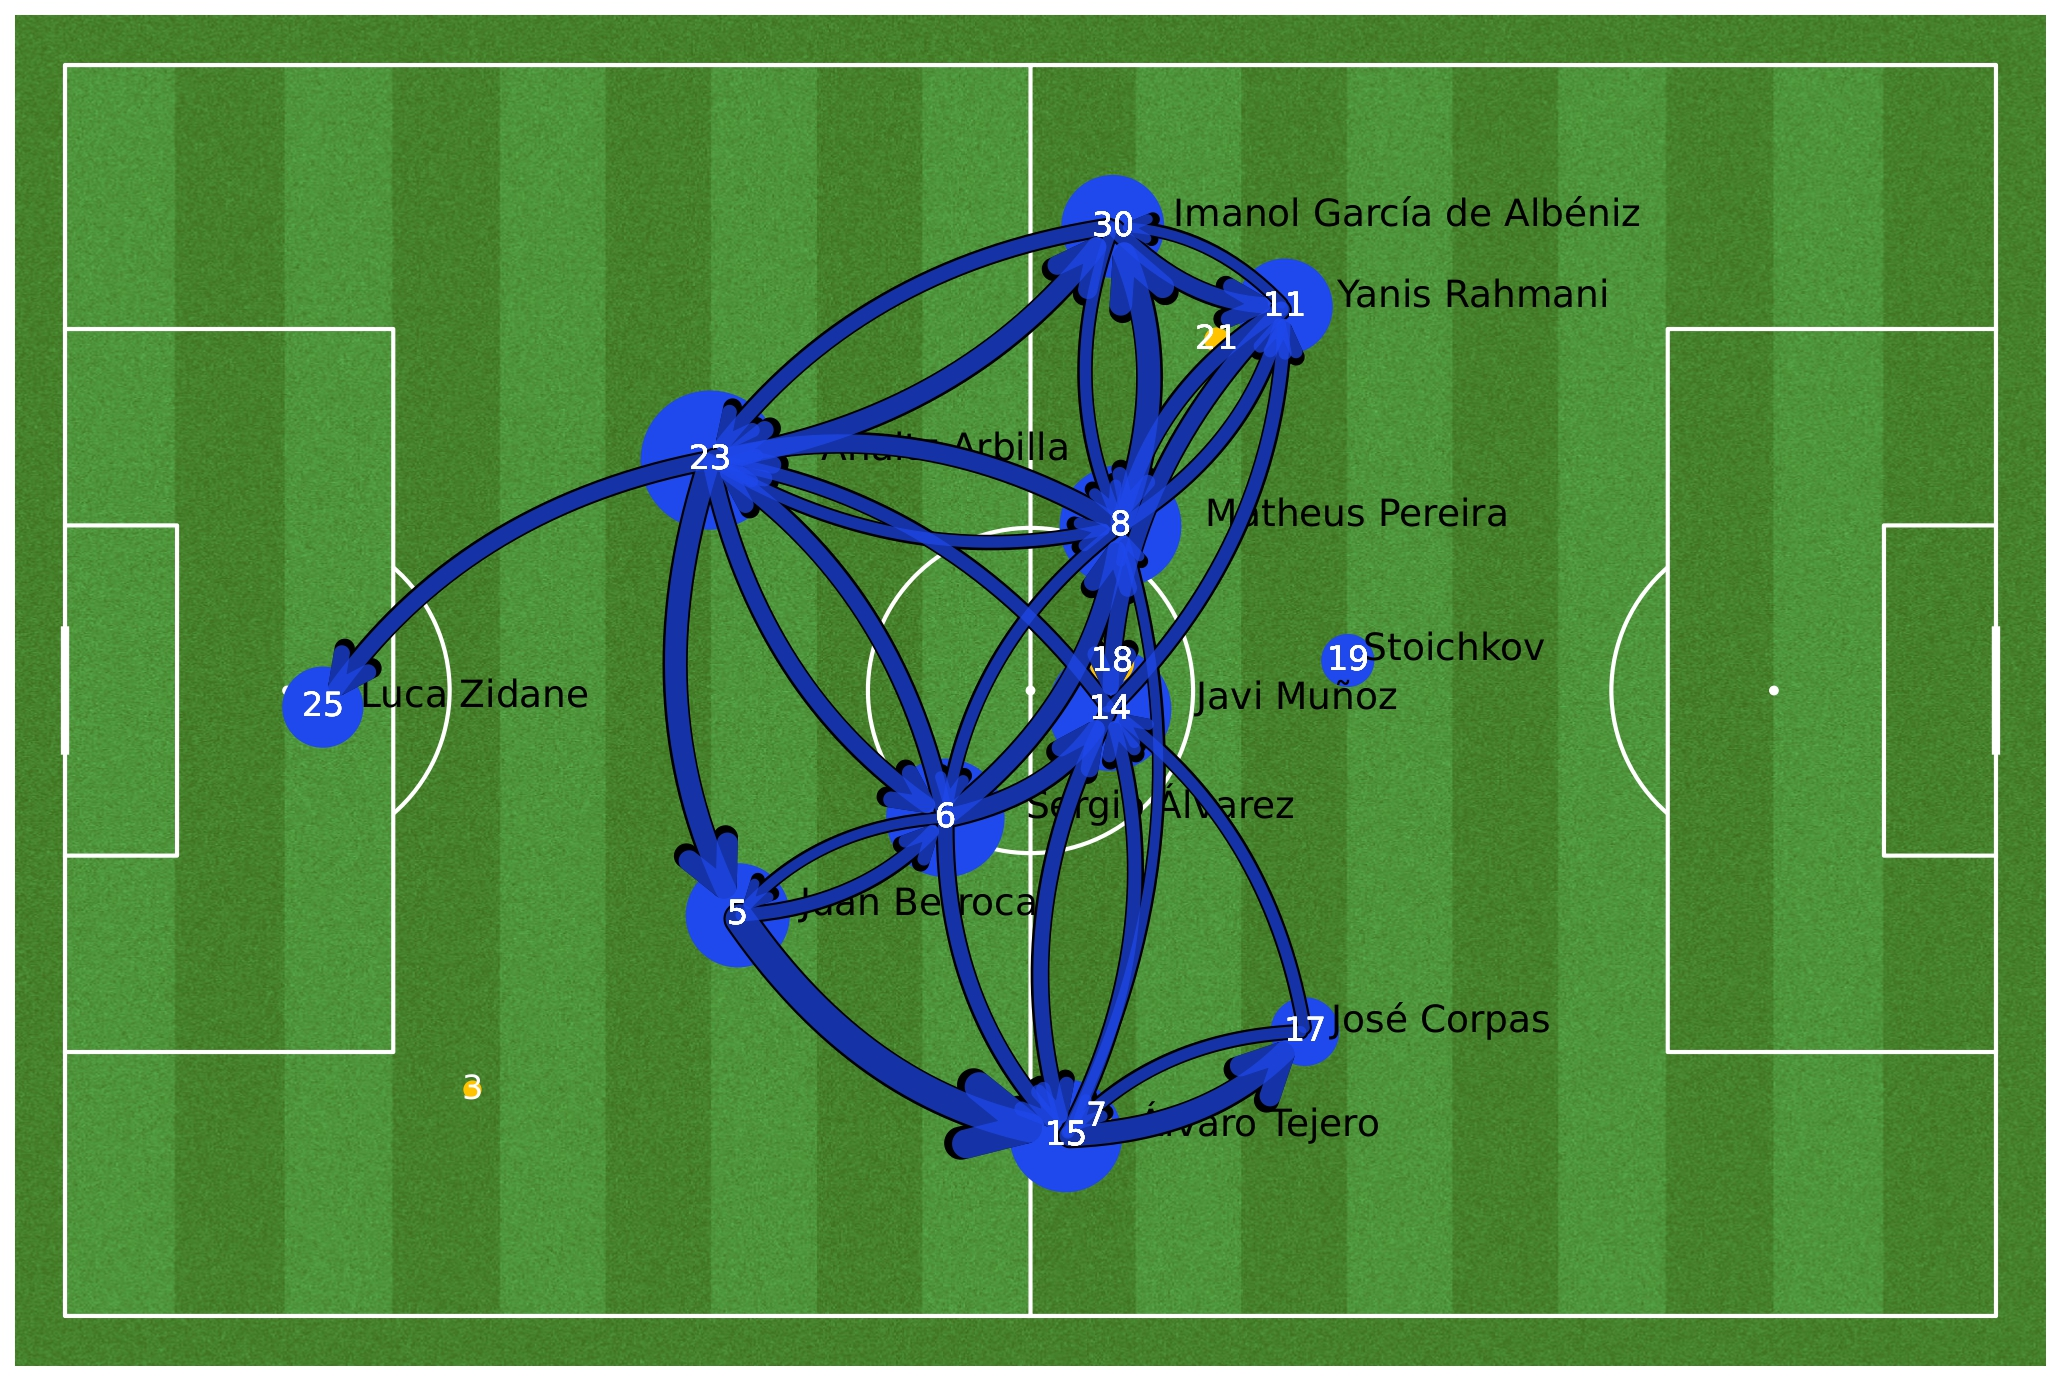
\includegraphics[width=0.5\linewidth,]{imagenes/home_pass_network} 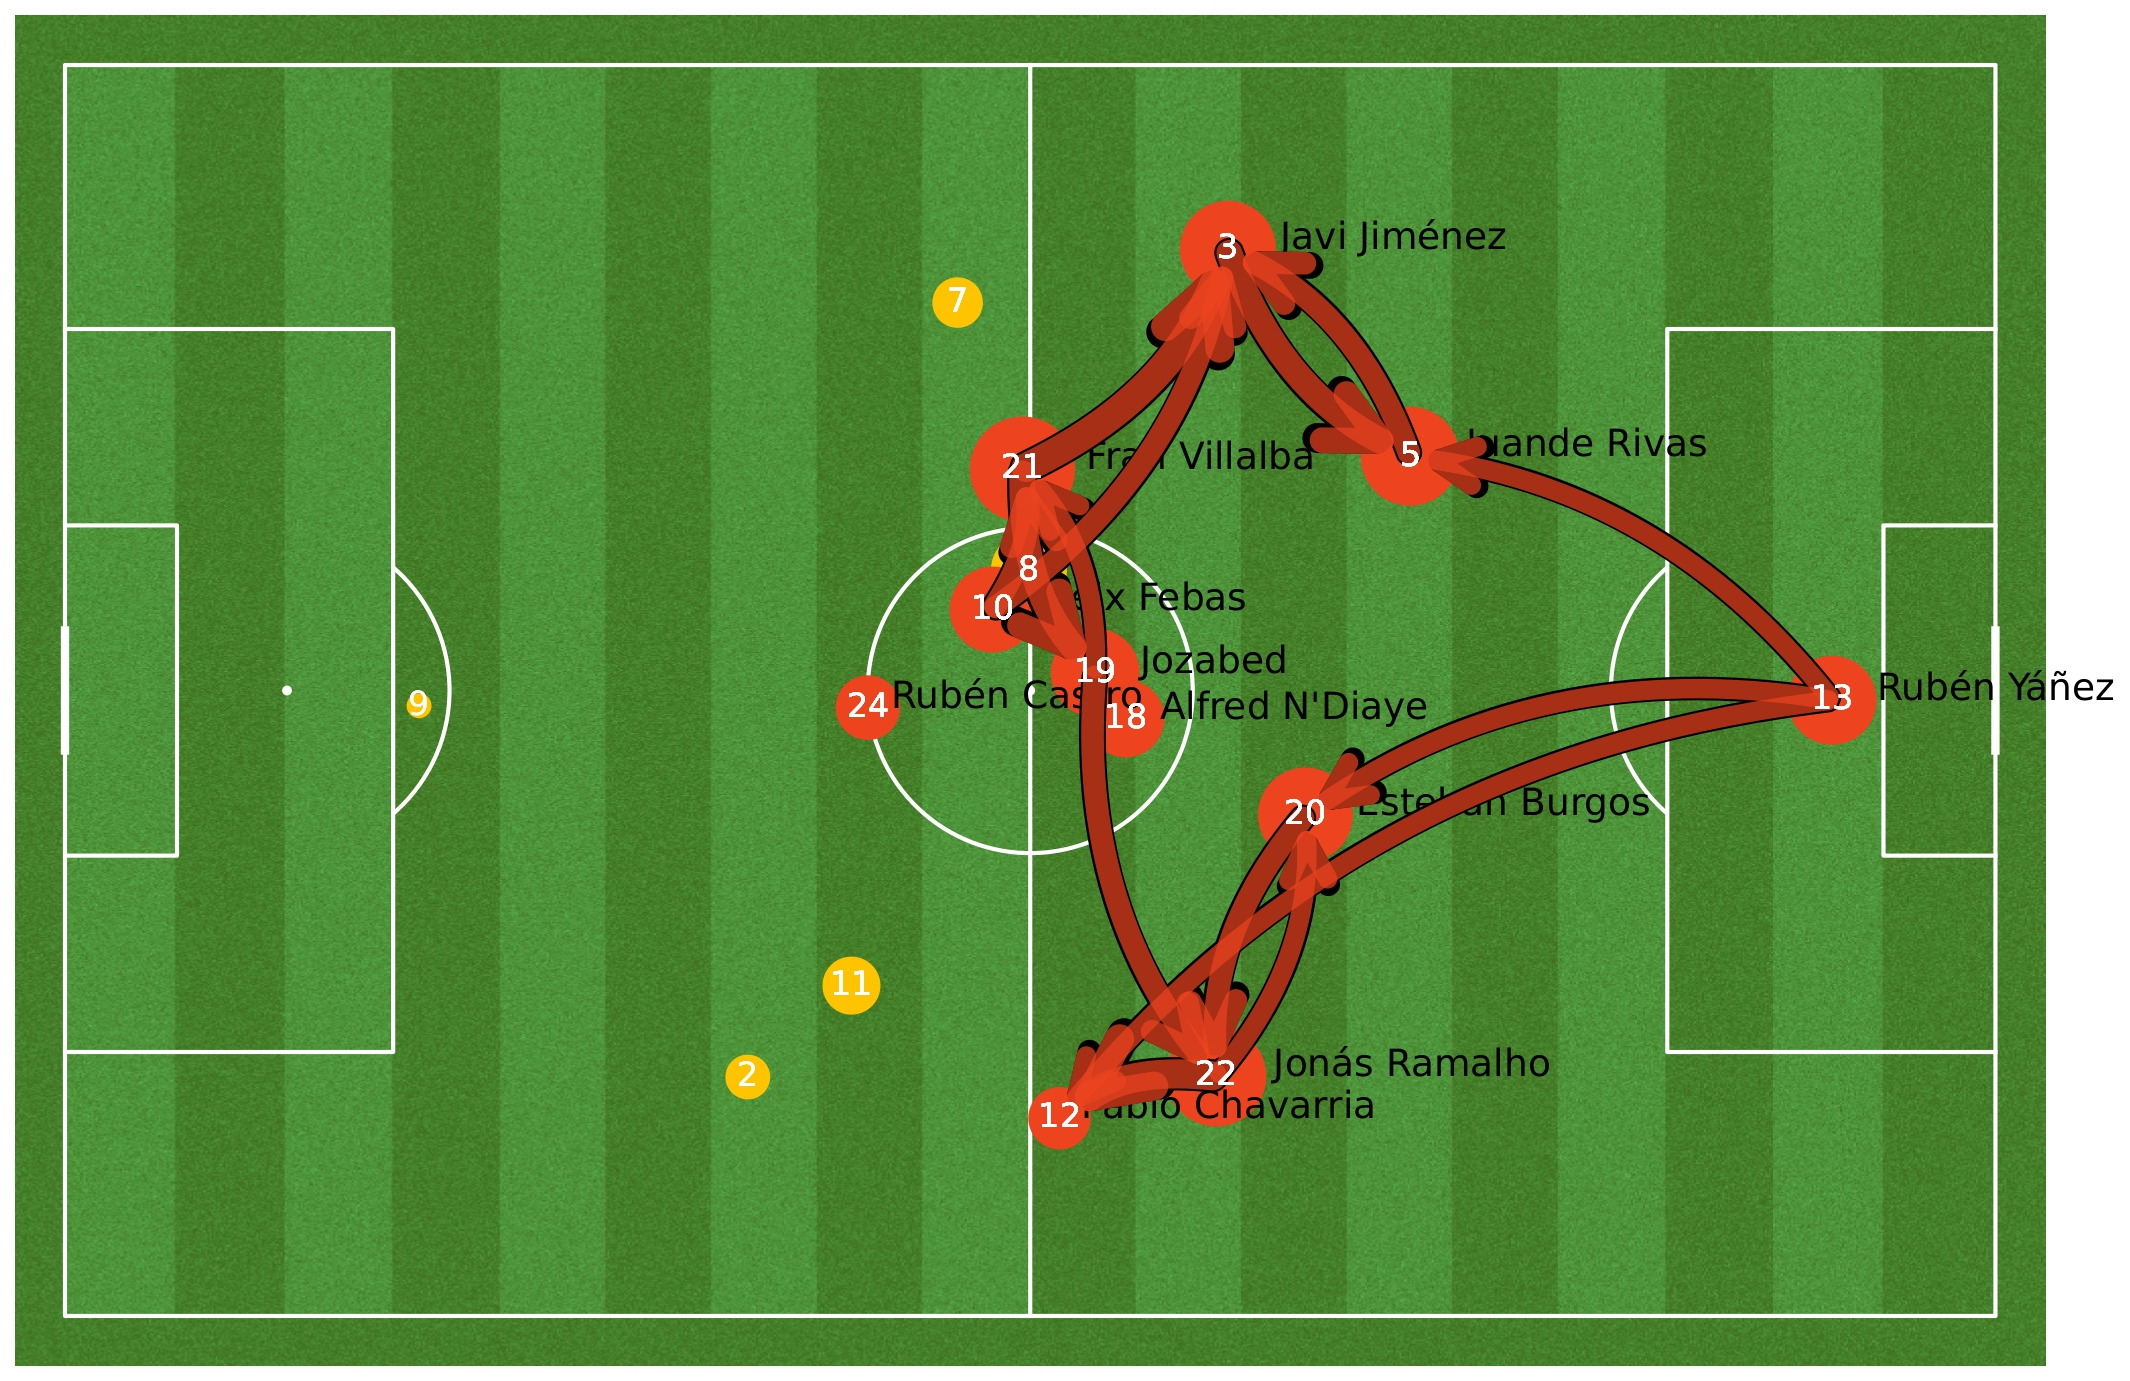
\includegraphics[width=0.5\linewidth,]{imagenes/away_pass_network} 

}

\caption{Representation of the Eibar (blue, left), Málaga (right, red) passing networks of the match Eibar - Málaga. Nodes represent players, edges represent passes between players. The position of the players in the field is their average passing position. The size of the nodes reflects the number of ingoing and outgoing passes (i.e. node’s degree), while the size of the edges is proportional to the number of passes between the players. Substitutes are represented in yellow. A connection is set if those players share at least 5 passes. The edge’s width is proportional to the amount of passes made in that direction between the two players.}\label{fig:homepass}
\end{figure}

Analysis as the former can be conducted \emph{in real-time}\footnote{Opta uses a combination of human annotation, computer vision, and
  AI modelling to offer real-time data at various levels of detail
  based on customer requirements. In our situation, the data feed
  updates itself when an event such as a goal, foul or pass occurs.
  Otherwise, it updates every 90 seconds. \citep{opta}} during the
match using appropriate data sources. Additionally, we could examine
Eibar's macro situation during the 2022-2023 season to better comprehend
how this micro-statistics contribute to the overall perception of the
team.

Fig. \ref{fig:xg-xga} presents the expected goals (xG) produced by Eibar in all matches played against their opponents. It is noticeable that Eibar has generated a higher xG when playing at their Home stadium, on average. In Fig. \ref{fig:rank-xg-xga} an overview of Eibar's performance against other teams in the Second Division is presented. It can be observed that Eibar ranks third in generating xGs against their opponents.

\begin{figure}[H]

{\centering 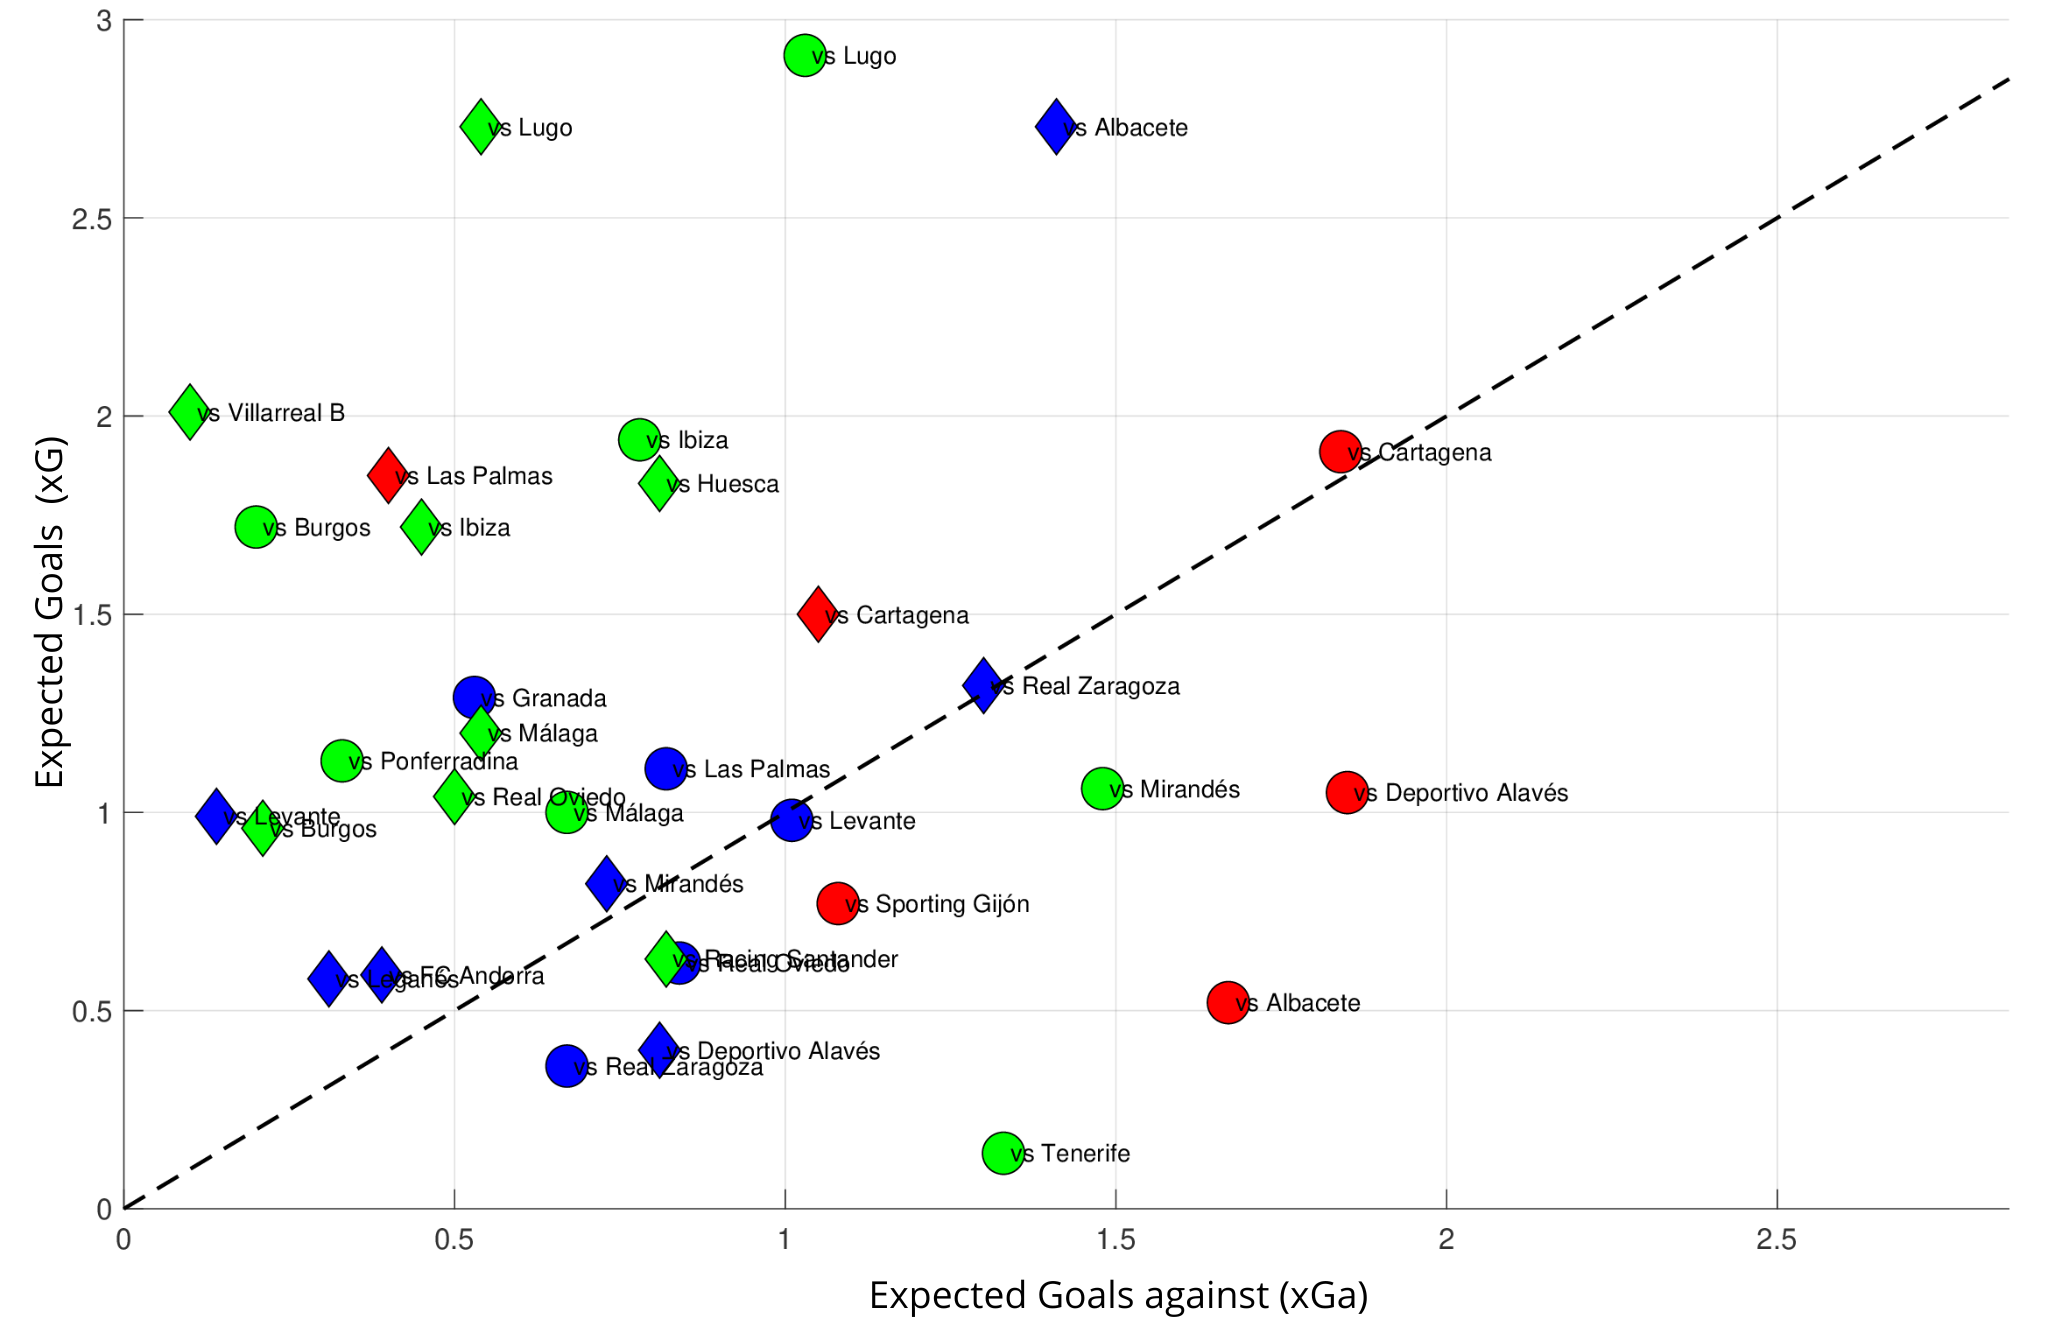
\includegraphics[width=0.8\linewidth,]{imagenes/scat-xG-xGa} 

}

\caption{Expected Goals (xG) and Expected Goals Against (xGA) per match. Codes: Home Matches (Diamonds), Away Matches (Circles), Wins (Green), Draws (Blue), Losses (Red). Matches above the dashed lines represent those matches where Eibar has generated more xG than the opponent.}\label{fig:xg-xga}
\end{figure}

\begin{figure}[H]

{\centering 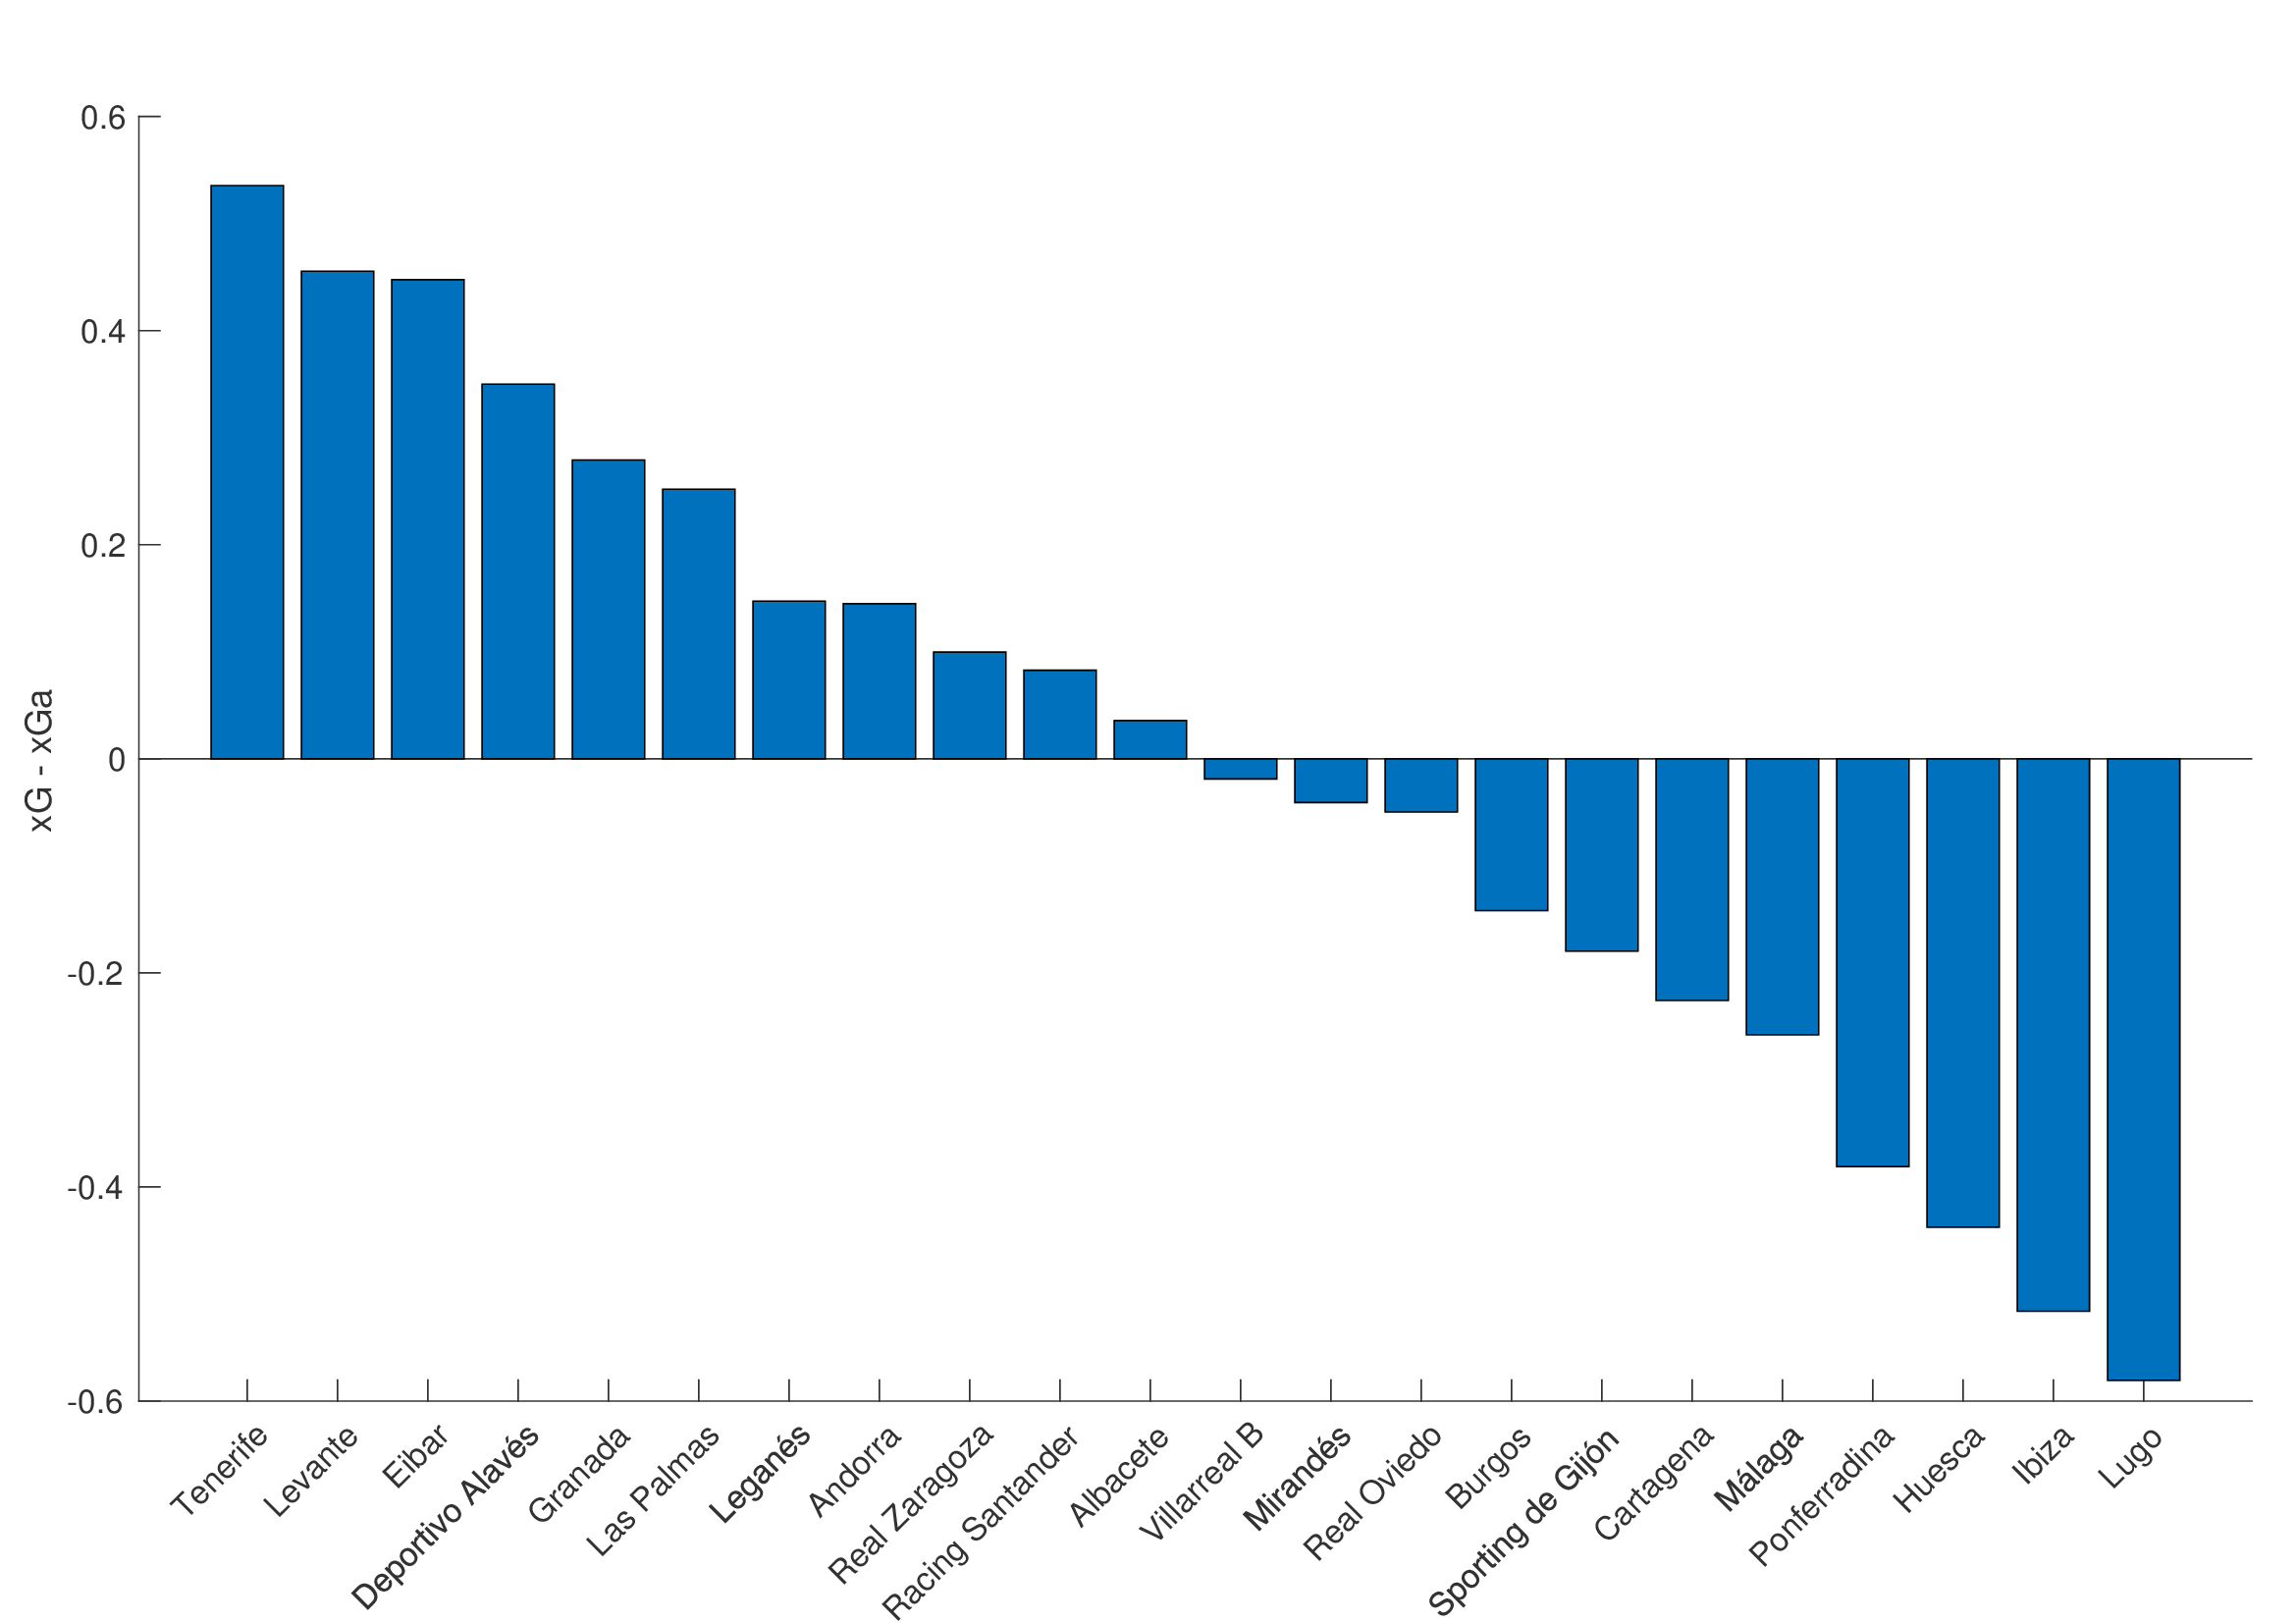
\includegraphics[width=0.8\linewidth,]{imagenes/xG-xGa} 

}

\caption{Ranking of the average differences in Expected Goals Scored (xG) Minus Expected Goals Conceded by Opponents (xGa) per team.}\label{fig:rank-xg-xga}
\end{figure}

We've just discussed some of the many statistics that can be inferred from this data sources to characterize the team performance, such as possession, pressure, duels, fouls, etc. This type of datasets are both easily manageable, and provide teams with useful information. Due to limitations in space and scope, however, we are unable to provide a more in-depth analysis of these measures

Although event datasets supply beneficial information regarding the team's overall performance, deeper scrutiny can be conducted via tracking data, which consists of the players' and ball's position and movement during the match. Tracking data can offer additional insight into both the physical and tactical aspects of the game.

\section{Tracking data}\label{tracking-data}

\texttt{Tracking\ data} offers a more comprehensive perspective than event data by providing access to information on all players, their trajectories, and velocities. This allows for the analysis of off-ball players and team dynamics, resulting in a more nuanced understanding of the game.

There are two main techniques for obtaining tracking data, which decide its classification: \textbf{Image detection algorithms} extract players' positions from the match broadcast and infer locations of concealed players, whereas \textbf{optical tracking} employs a specialized camera system installed on the field to record players' data. Our research will concentrate on the latter method, as it offers more precise and statistically informative data.

Our tracking data has been provided by Mediacoach®. They utilises the Tracab Optical Tracking system to obtain on-the-pitch player positions. This multi-camera system captures each player's position at 25 frames per second. The system consists of three units, each with a resolution of 1920x1080 pixels, producing a panoramic picture that generates a stereoscopic view for triangulating the players and ball. In case of a temporary loss of any location, a skilled operator adjusts the players' positions. The datasets obtained by the Mediacoach® system have been validated in advance using GPS \citep{Felipe2019ValidationOA}.

Fig. \ref{fig:frame} contains a frame from the tracking dataset of an Atlético de Madrid (Blue) - Getafe (Red) game from the Spanish 2019 League. The ball is shown as a black dot. Referees are shown as yellow squares. Purple arrows represent the speed vectors of the players.

\begin{figure}[H]

{\centering \includegraphics[width=0.8\linewidth,]{imagenes/Frame} 

}

\caption{A frame of tracking data from a football match. The home team is shown in blue, the away team in red. The ball is shown as a black dot. Referees are shown as yellow squares. Purple arrows represent the speed vectors of the players.}\label{fig:frame}
\end{figure}

Traditionally, all football statistics have been produced using event datasets. In this respect, tracking datasets have been crucial in developing new ways of measuring team and player performance. With this type of information, we are not just limited to ball-related events such as passes, goals, etc. tracking datasets contain the precise location of players and the ball during a match. \citep{GARRIDO2022112827} showed that the correlation between heatmaps, Fig. \ref{fig:heatmap}, made with event datasets and those made with tracking datasets is low. Event heatmaps show where a player has performed more actions. On the other hand, tracking heatmaps provide information about a player's position without adding information about how relevant his about how relevant their performance was.

\begin{figure}[H]

{\centering \includegraphics[width=0.8\linewidth,]{imagenes/Heatmap} 

}

\caption{Heatmap of the ball position during the Atlético de Madrid - Getafe game under study. Note that we always keep the direction of play from left to right, so the home team will always be placed on the left side of the field and the away team on the right.}\label{fig:heatmap}
\end{figure}

Thus, tracking datasets are crucial for developing new ways of measuring team and player performance, as they provide us with global information about the game.

This data-driven approach enhances the understanding of the sport and its strategic nuances, fostering a deeper appreciation of the game's intricacies. As a result, tracking data has become a valuable tool in football analysis, providing insights into player performance and team strategy. These advanced metrics can be applied to specific games, as in the analysis presented earlier (Fig. \ref{fig:heatmap}), or to an ensemble of them to provide a comprehensive view of general player behavior under different parameters. In the following section, we will introduce two main frameworks from which our present a selection of these metrics, both physical and tactical, to provide context for our proposed offside control metric across multiple games.

After the initial review of the state of art of football analytics, we will introduce the methodology behind our proposed metric to characterize offside strategy's effectiveness. In this chapter, we will combine both physical metrics and tactical models derived from Tracking datasets to build the proposed metric: \emph{Offside Control}

\chapter{Methodology}\label{methodology}

As discussed earlier, tracking datasets provide the position of all players and the ball throughout the match with a temporal resolution of 25fps. This enables us to estimate the players' covered distance, speed, and acceleration. The potential for extracting information from tracking datasets that is useful for football analytics extends beyond variables related to players' physical performance. Many tactical metrics has been implemented to decode how the intricate movements of players translate to the soccer field.

These models provide a scientific perspective for analysing player positioning, decision-
making, and team dynamics, illuminating the complex interactions that occur during a
match.

\emph{Pitch Control} is one of the most relevant tactical metrics used to analyse player positioning, decision-making, and team dynamics during a soccer match. It combines player position and speed with mathematical models that simulate ball and player movement \citep{Spearman}.

This master's thesis proposes using Pitch Control Models to evaluate how football teams interact with the offside line when attacking and defending. Before that, we need first to define and understand Pitch Control Models, including their construction and implementation.

\section{Pitch Control Models}\label{pitch-control-models}

The \emph{Pitch Control (PC)} at a given location represents the probability of a player or team gaining control of the ball if it moves directly to that location. \emph{PC} models simulate the dynamics of the ball and the players to evaluate which player would control the ball if it moves to any location on the pitch at any moment.
The model captures not only the players' current position, but also their movement. When players are running at high speeds, they are more likely to control
the space they are moving into rather than the space they currently occupy.

To construct this model, we must calculate the following for a given location on the pitch:

\begin{itemize}
\tightlist
\item
  How long it would take for the ball to reach to the position of interest (from its starting position).
\item
  How long would it take for each player to get to that position.
\item
  What is the total \emph{probability} that each team will control the ball \emph{after} both the players and the ball have arrived at the desired position?
\end{itemize}

In the model, the ball is set to move at a constant speed of \(v_b = 54\) \(km/h\), which is approximately the average speed of the ball in the game (See Fig. \ref{fig:ball})

\begin{figure}[H]

{\centering 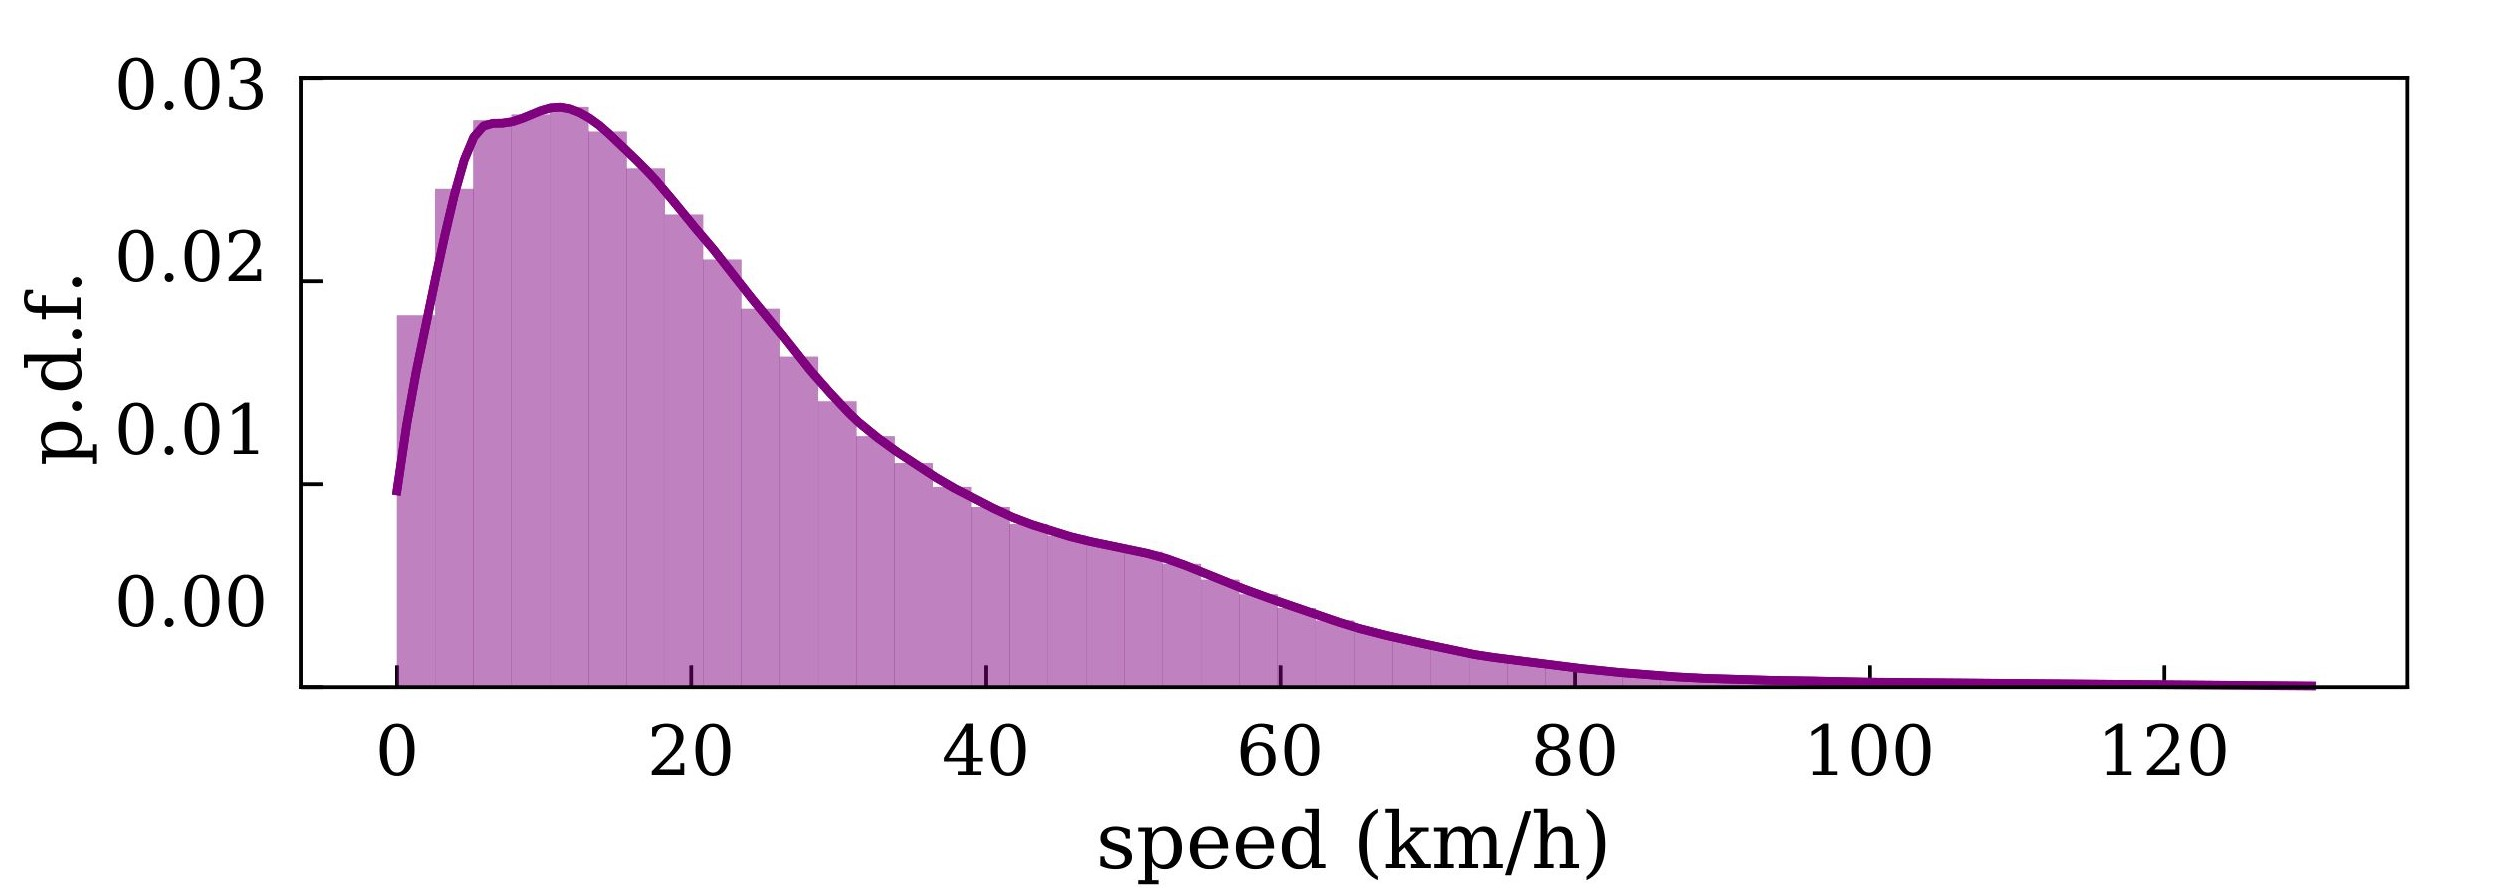
\includegraphics[width=0.8\linewidth,]{imagenes/ball} 

}

\caption{p.d.f of the ball speed over a 100 matches from LaLiga 2019-2020 season.}\label{fig:ball}
\end{figure}

Therefore, the time taken to arrive at the location of interest can be easily calculated as \(t_{b,arr} = \Delta x_b/v_b\), where \(\Delta x_b\) is the distance between the initial and final positions of the ball.

\subsection{Model assumptions}\label{model-assumptions}

When considering how long it will take the players to reach the target position, given their initial position and speed, players are assumed to only have a maximum speed of \(v_{max,p} = 18\) \(km/h\), which corresponds to the 95 percentile of the average speed of the players in the game (See Fig. \ref{fig:vel}). This upper limit should not be misunderstood as the maximum speed at which players can move, but rather as an estimate of the maximum speed at which they are likely to move when trying to control the ball

\begin{figure}[H]

{\centering 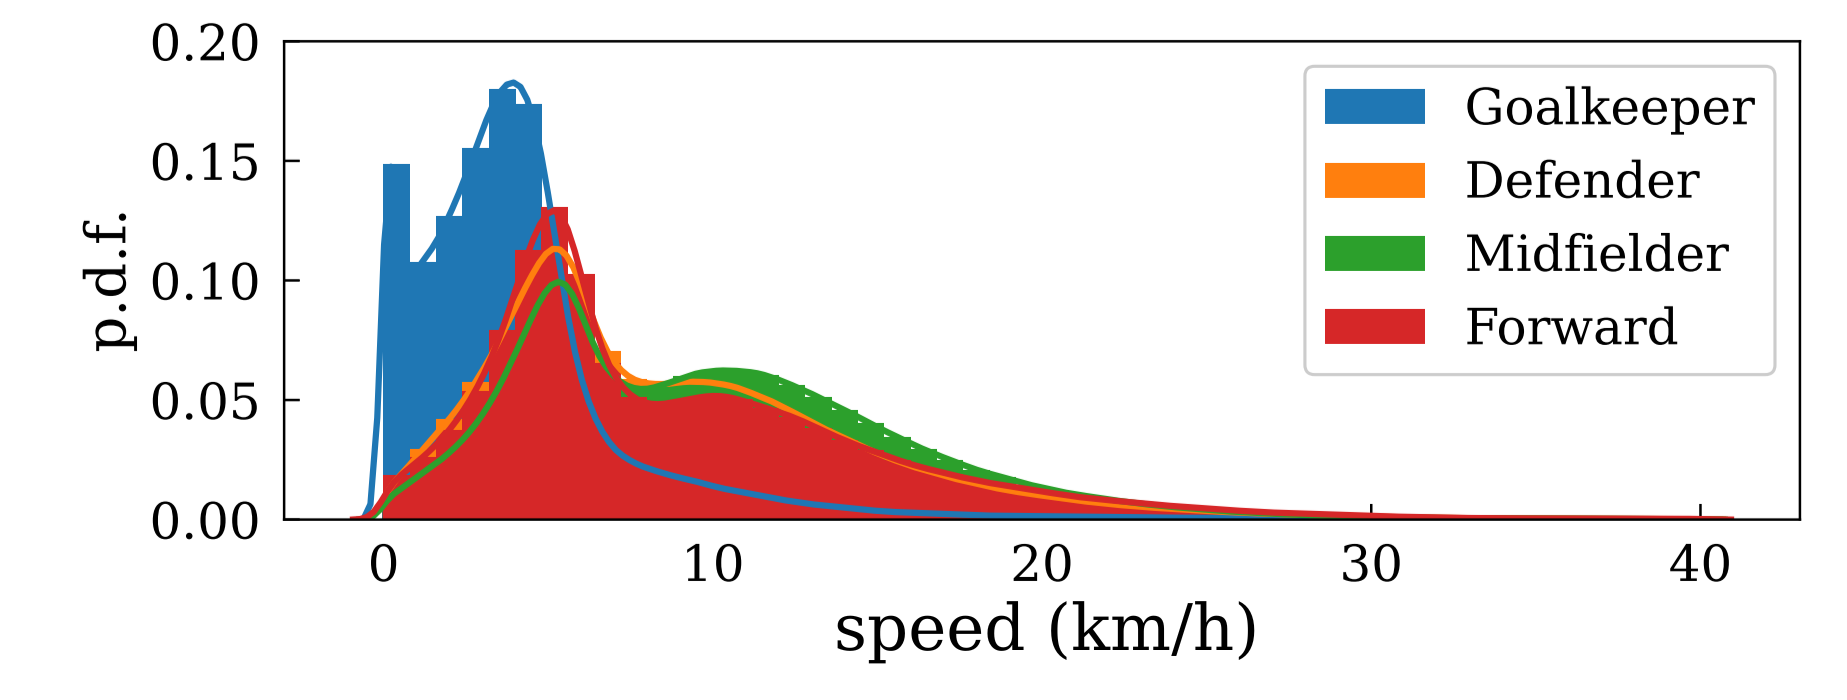
\includegraphics[width=0.8\linewidth,]{imagenes/vel} 

}

\caption{p.d.f of the players speed over a 100 matches from LaLiga 2019-2020 season.}\label{fig:vel}
\end{figure}

To compute the player's expected arrival time, \(\tau_{exp}(\vec{r};t_r)\) , we use a simple approximation consisting of a two-step process:

\begin{itemize}
\tightlist
\item
  There is an initial \emph{reaction time}, assumed to be of \(t_{r} = 0.7\) seconds for every player\footnote{We can impose this assumption for all the players without loss of generality, to simplify the model. Further work to improve the model will be individualize this reaction parameter for each player.}. This is approximately the time it takes a player moving at maximum speed to come to a complete stop. During this reaction time, we assume that players continue to move along their current trajectory without changing speed or direction (reaching a position \(\vec{r}_{\text{react}}\)).
\item
  After this time, we assume that the player runs directly towards the ball at his maximum speed of \(v_{\text{max,p}}\).
\end{itemize}

\begin{align}
    \tau_{exp}(\vec{r} ; t_r) = t_r + \frac{|\vec{r} - \vec{r}_{react}|}{v_{max,p}}
    \label{exp_arr_time}
\end{align}

\subsection{Control probability}\label{control-probability}

Once we computed the time it takes for the ball and the players to get to the target location, we need to look at how long it will take each player to control the ball. To do so, we will assume that controlling the ball is a stochastic process that follows an exponential distribution with a fixed rate \(\lambda\), with units of \(1/s\). Thus, for any differential time \(\Delta t\) that a player is near the ball, he has a probability of \(\lambda \cdot \Delta t\) of controlling the ball.

\begin{align}
F(\Delta t ; \lambda)=1-e^{-\lambda \Delta t}
\end{align}

So far, the model assumes that we know exactly when each player will arrive at the target location. However, we introduce some uncertainty, labelled \(\sigma\), in the arrival time of the players. The reason for including such temporal variability in our model is to account for some effects that have not been explicitly modeled, such as player effort. Thus, the probability of a player intercepting the ball at time T is given by the cumulative distribution function of the sigmoid distribution (See Fig. \ref{fig:lambda}).

\begin{align}
    F_{\text {int }}(\vec{r},T;\sigma, t_r)=\frac{1}{1+e^{-\frac{T- \tau_{exp}(\vec{r} ; t_r)}{\sqrt{3} \sigma / \pi}}}
    \label{sigmoid}
\end{align}

\begin{figure}[H]

{\centering 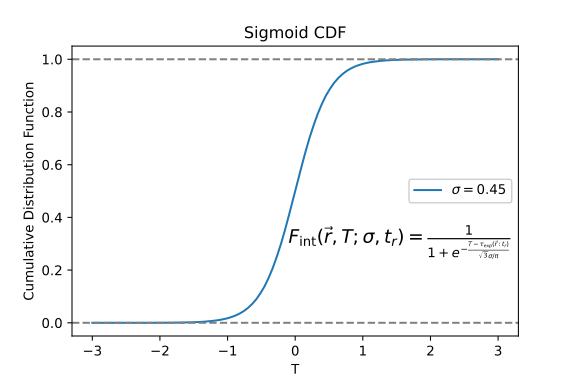
\includegraphics[width=0.45\linewidth,]{imagenes/sigmoid_poster} 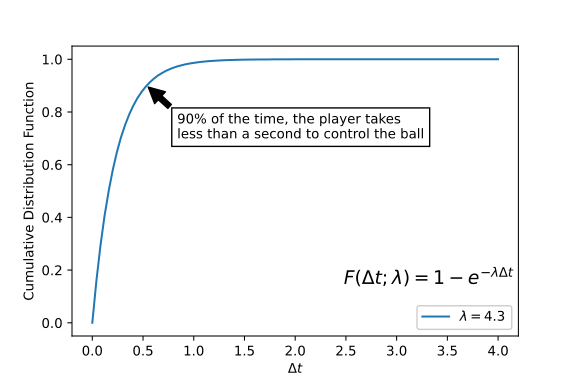
\includegraphics[width=0.45\linewidth,]{imagenes/exp_poster} 

}

\caption{The cumulative distribution functions for the two components of the model. a) (left) the time to intercept and b) (right) the time to control the ball.    The parameters shown for each are from the global fit described below.}\label{fig:lambda}
\end{figure}

Both \(\lambda\) and \(\sigma\) has been selected according to \citep{SpearmanFit}, where they model passes as a Bernoulli trial, with probability mass function

\begin{align}
P(k \mid \sigma, \lambda, x)=\left\{\begin{array}{lr}
1-p \text { for } \mathrm{k}=0 \\
p & \text { for } \mathrm{k}=1
\end{array}\right.
\end{align}

where \(k \in [0,1]\) is the outcome of the pass. Then, the likelihood of a set of\\
parameters, \(\sigma\) and \(\lambda\), given outcome \(k\) and the start of the pass \(x\) is:

\begin{align}
\mathcal{L}(\sigma, \lambda \mid k, x)=P(k \mid \sigma, \lambda, x)
\end{align}

Then, maximizing the product of the likelihood for each pass for a training sample P, the best fit is found at \(\sigma=0.45 \pm 0.05 \mathrm{~s} \text { and } \lambda=4.30 \pm 1.14 \mathrm{~s}^{-1}\)\footnote{See \citep{SpearmanFit} for further details}

\begin{align}
\min _{\sigma, \lambda \in\{\mathbb{R}, \mathbb{R}\}}\left\{-\sum_{i \in P} \log \left[\mathcal{L}\left(\sigma, \lambda \mid k_i, x_i\right)\right]\right\}
\end{align}

Using the above components, we recursively construct the partial derivative of the probability that player \(j\) controls a given location \(r\), at time t is

\begin{align}
\frac{d P P C F_j}{d t}\left(T, \vec{r} , \sigma, \lambda_j, t_r\right)=\left(1-\sum_k P P C F_k\left(t, \vec{r} , \sigma, \lambda_k\right)\right) F_{int,j}(t, \vec{r}  , \sigma, t_r) \lambda_j
\label{eq:PC}
\end{align}

where \(PPCF_j\) is the Potential Pitch Control Field of player \(j\). \(F_{int,j}(t, \vec{r}, T ; \sigma, t_r)\) is the probability that player \(j\) can reach the target location \(r\) in a given time \(t\), and \(\lambda_j\) is the control rate of such a player \footnote{We assign the goalkeepers to have a higher control rate, \(\lambda_{GK} = 12.9\) \(s^{-1}\), to ensure that they are likely to claim the ball if it is near them and also to account for the ability of grabbing the ball with their hands}. Importantly, note that \(\sum_k P P C F_k\left(T, \vec{r} , \sigma, \lambda_k\right)\) accounts for the sum of the Potential Pitch Control Field of the rest of the \(k\) players on the pitch at time \(t\).

By integrating the equation above, Eq. \eqref{eq:PC}, \(t \in \left[ t_{ball},t_{ball} + 10 \right]\) seconds, and taking \(P P C F_j\left(t, \vec{r} , \sigma, \lambda_j\right) = 0\) at the beginning of the integration, the probability of control per player is obtained. This probability is then extracted along all the pitch, obtaining a pitch control surface.

Now that we are able to generate the pitch control surface for a frame, we can extend this methodology to measure the quality of each team's offside strategy. To do this, we will focus on the pitch control generated \emph{after} the offside line, called \textbf{Offside Control (OC)}. To do this, we determine where the offside line is and which players are in an offside position. Then we calculate the pitch control generated by the attacking team after the offside line. If a player is in an offside position, we mark his contribution as ineffective.

The \emph{Offside Control} was calculated for 100 matches from LaLiga (season 2018 - 2019) using tracking data. We calculated the OC every 2 frames per second of each match. In order to discretise the space efficiently, we decided to reduce our calculations to the half of the pitch of the team not in possession of the ball. We then detect the position of the offside line and calculate the pitch control after it. In this way, we significantly reduce the computation time of the model while maintaining a high spatial resolution (\(50 \times 32\)).

\chapter{Offside Control}\label{offside-control}

As previously mentioned, this master's thesis introduces the parameter \emph{Offside Control (OC)}, which is derived through a modification of the Potential Pitch Control Field methodology. The purpose is to examine the pitch control dynamics of teams or individual players after the offside line. The procedure involves first identifying the offside line, which is determined by the positioning of the second-to-last defender. Identify attacking players who are within permissible boundaries and in offside positions across each frame. Calculate the OC metric as the measure of pitch control exerted by the attacking team or player subsequent to the offside demarcation. Additionally, assess the involvement of a player in an offside position as a manifestation of ineffective Offside Control (IOC). Conversely, instances where a player is positioned beyond the offside line and maintains control of the ball are classified as effective Offside Control (EOC).

We presented this metric at \emph{OptaForum 2023}, which took place in central London on Tuesday 21 March. Our proposal was one of only 5 selected to be included in the congress. It was a privilege to learn from other leading experts in the field, and also generated fruitful conversations that were fundamental to the development of the work\footnote{You can check the rest of the proposals accepted here \url{https://www.statsperform.com/resource/first-presentations-announced-for-the-2023-opta-forums-pro-track/}}.

\section{Results}\label{results}

The concept of effective and ineffective Offside Control is illustrated in Fig. \ref{fig:eff}. Players from both teams are shown in blue (home team, attacking from left to right) and red (away team, attacking from right to left). Areas of the pitch controlled by the home team are shown in blue, while areas controlled by the away team in that particular match are shown in red. In this frame, the home team is in possession of the ball. The vertical dashed line indicates the position of the offside line. The areas surrounded by a broad grey line represent the areas controlled by the attacking team behind the offside line. We can see that the home player with the number \(11\) is behind the offside line, in an invalid position, and therefore generates IOC around him. On the contrary, player \(18\) is in a correct position and the Offside Control generated behind the offside line is classified as effective (EOC).

The \emph{Spatial Offside Control} generated by a team can be obtained by simply summing the Offside Control of each team during the match in each region of the pitch behind the offside line. We can also define the \emph{Percentage of Offside Control} accumulated by each team and obtain an indicator of which team gained more control over the opponent. Fig. \ref{fig:games} shows two examples of both spatial OC and percentage of OC for two different games (A and B) by a team called \(\alpha\). We have used a heatmap to show in red the spatial OC generated and received by team \(\alpha\), indicating which specific areas of the pitch were controlled behind the offside line. Note that only effective Offside Control is shown in this example. We can see that in match \(A\) the danger generated behind the offside line is deeper and closer to the box, while the EOC received is not as close to the own goal. On the other hand, in game \(B\), the EOC generated is more longitudinal and closer to the edge of the pitch, while the EOC generated by the opposing team is much deeper and therefore more dangerous. Beyond the spatial location, the bars on the right side of the figure \ref{fig:games} show the proportion of EOC accumulated by team \(\alpha\) and its opponents in both games. In both cases, team \(\alpha\) dominates the opposing team, accumulating a percentage higher than \(65\%\).

\begin{figure}[H]

{\centering \includegraphics[width=0.8\linewidth,]{imagenes/eff_inef_OC} 

}

\caption{Example of effective (EOC) and ineffective (IOC) Offside Control (areas surrounded by a thick grey line). Offside is indicated by the vertical dashed line. Note that player $11$ is offside (generating IOC), while player $18$ is not (generating EOC).}\label{fig:eff}
\end{figure}

\begin{figure}[H]

{\centering 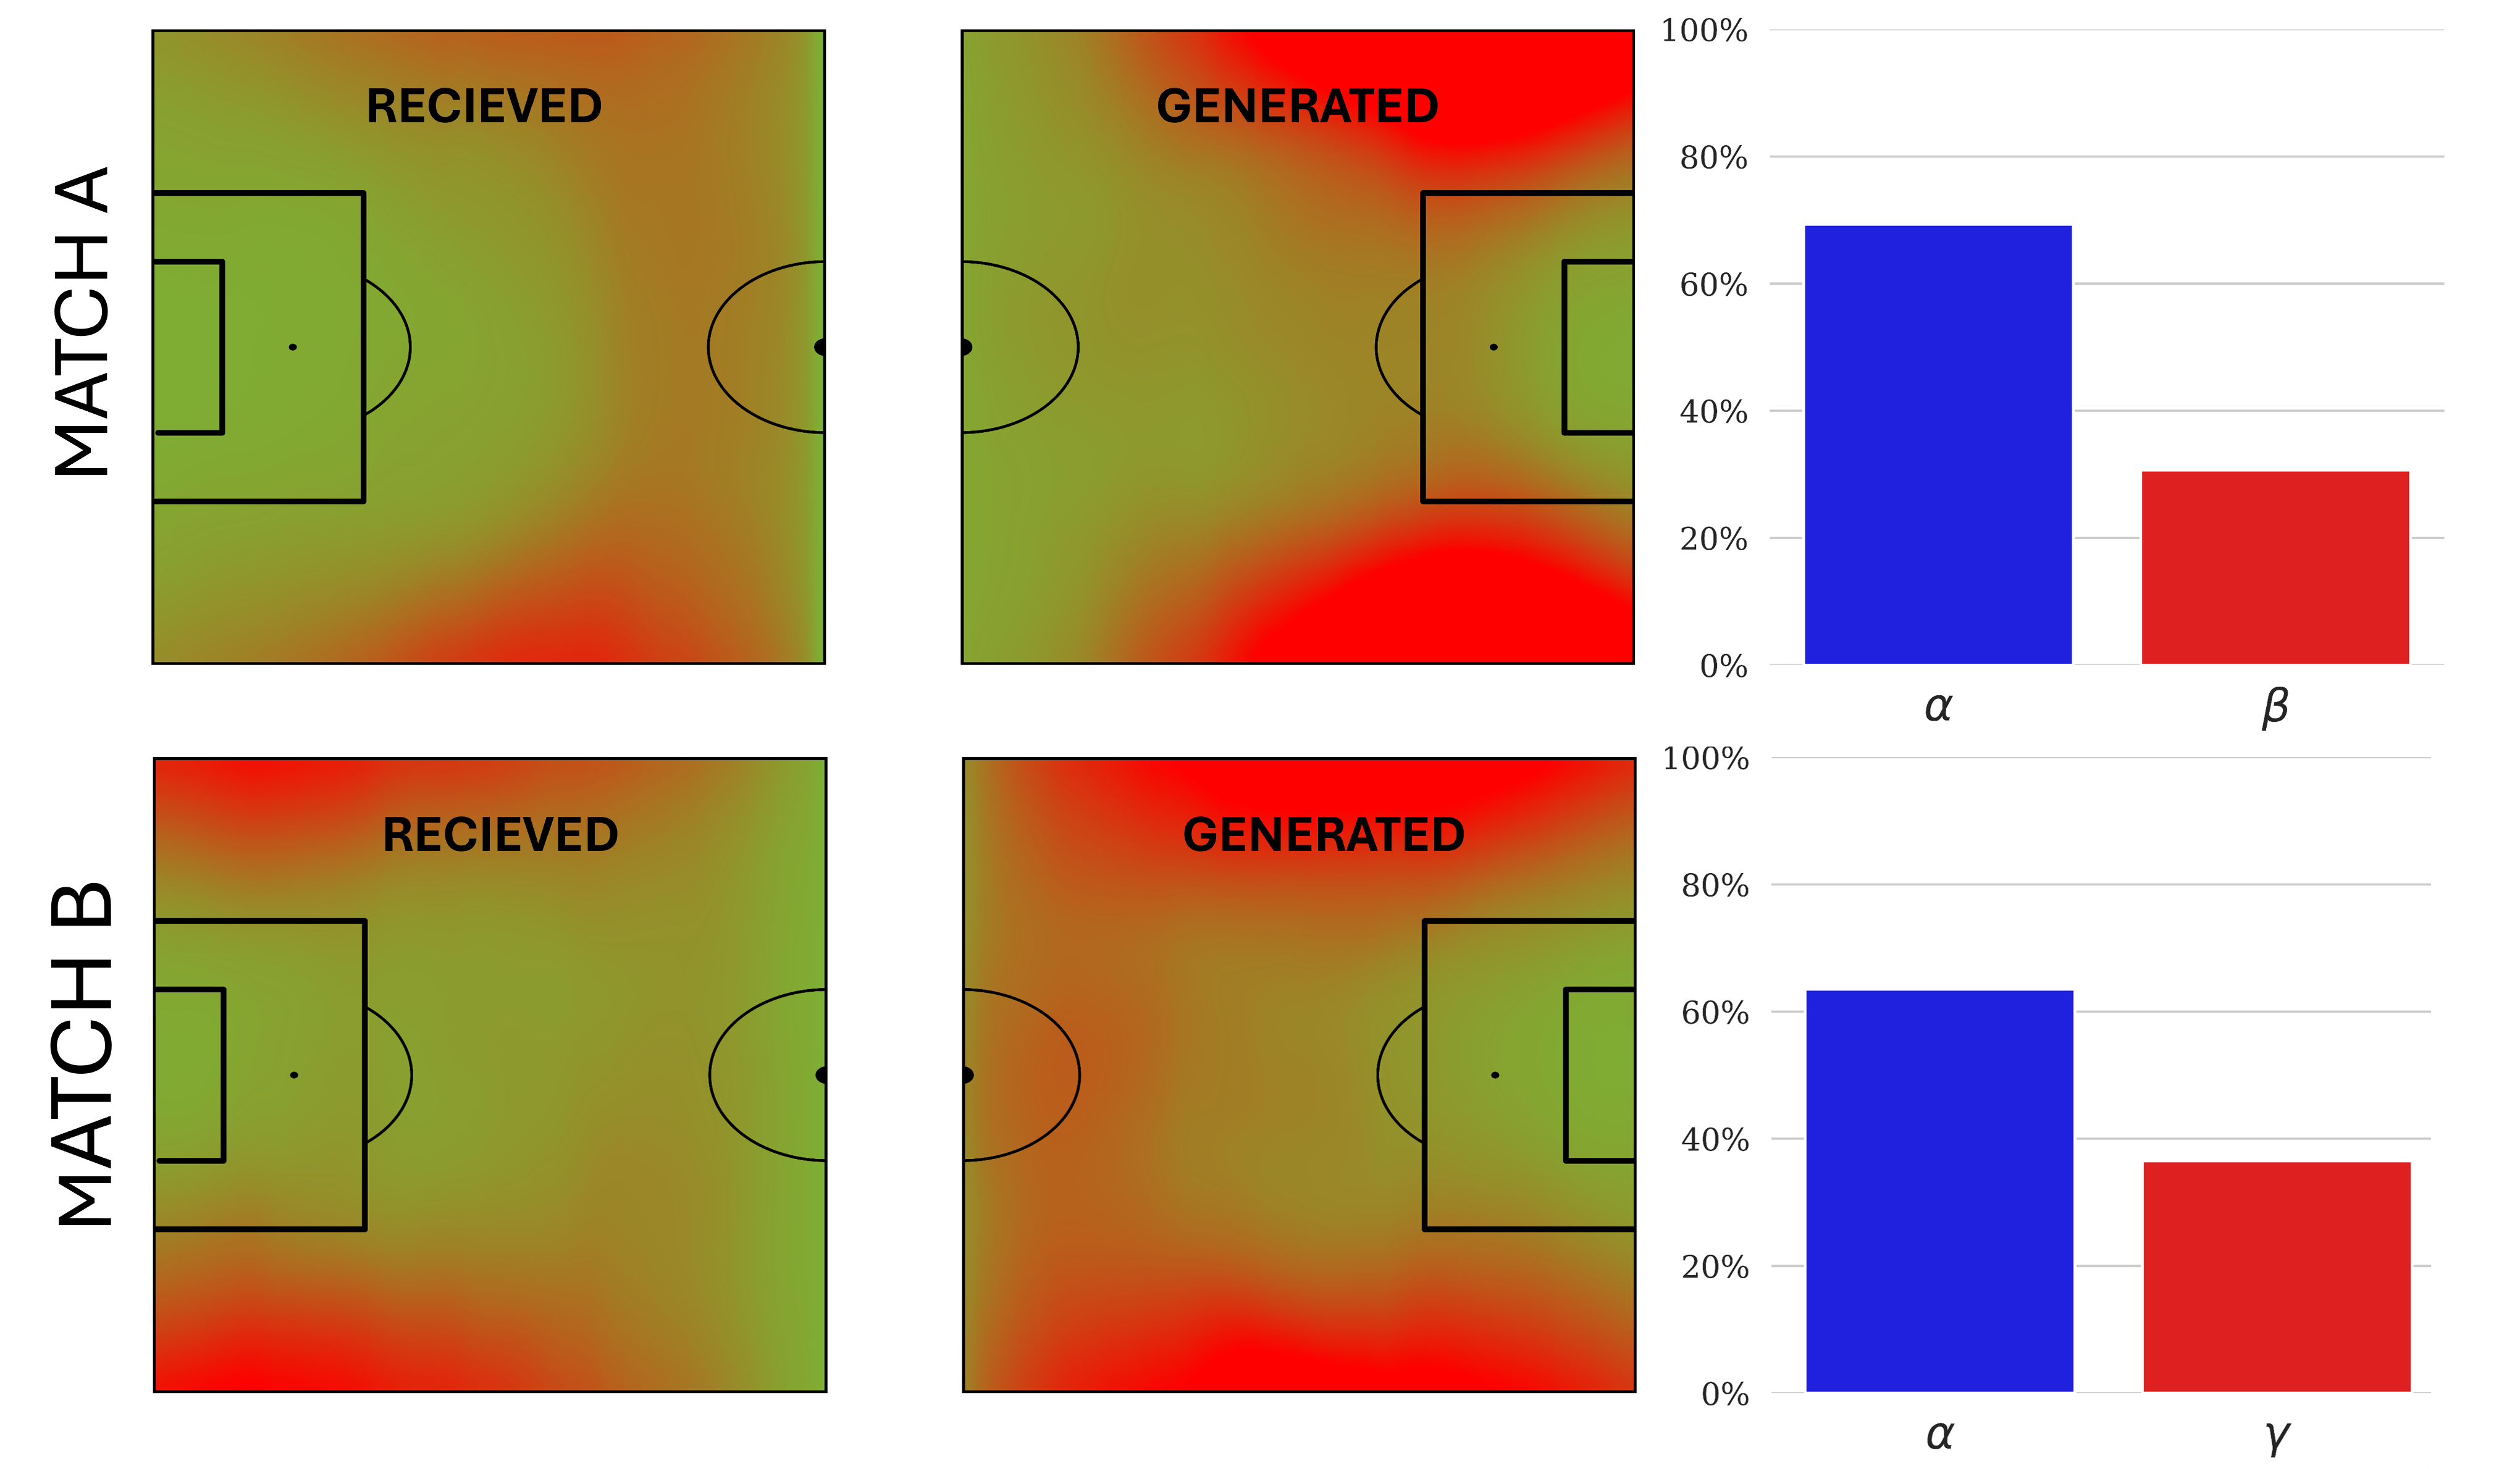
\includegraphics[width=0.8\linewidth,]{imagenes/Games_OC} 

}

\caption{Spatial and percentage of effective offside control (EOC) over the course of two matches (A and B). The left plots show the EOC received by team $\alpha$ and the middle plots show the EOC generated by team $\alpha$. In all plots, the intensity of the red color is proportional to the accumulated EOC at each location on the field. The bars on the right show the percentage of EOC accumulated by team $\alpha$ and its opponents.}\label{fig:games}
\end{figure}

Offside Control can also be tracked over the course of a match. Fig. \ref{fig:oct} shows an example of \(OC(t)\) for the home team of a match, smoothed with a centred sliding window of 600 frames. In the figure we have also included the moments when goals were scored. This allows us to relate the \(OC(t)\) to the score. As we have plotted the home team's \(OC(t)\), we can see that it increases until a few minutes before the third goal is scored. However, it drops around minute 50, which shows that the home team is creating less danger behind the opponent's offside line, presumably trying to defend the goal advantage rather than create new scoring opportunities.

\begin{figure}[H]

{\centering 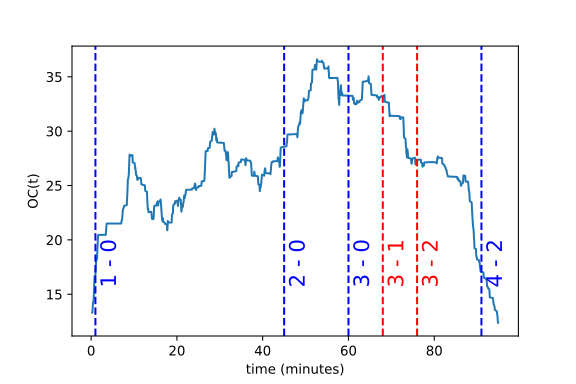
\includegraphics[width=0.8\linewidth,]{imagenes/cumulative_OC_evolution} 

}

\caption{Analysis of the home team's Offside Control over the course of a match. Each point of $OC(t)$ is calculated using a centred sliding window of 600 frames. The vertical dashed lines indicate the moments when a goal was scored (blue for the home team and red for the away team).}\label{fig:oct}
\end{figure}

After analysing the OC of the 99 games evaluated in the study, we can also analyse the OC performance of all teams in the competition. Fig. \ref{fig:ranking} shows a comparison between the generated and received OC per effective time unit, for all teams. In the figure, the size of the teams and their labels indicate the final ranking after the matches included in the analysis. The dashed line plotted (\(y=x\)) separates the teams with positive and negative differences between the generated and received OC. Thus, teams below the dashed line generate less OC than their rivals, while teams above it accumulate more OC than their opponents. We can also observe a slight negative correlation between the OC generated and the OC received, although the correlation coefficient \(R^2=0.48\) is relatively low. Note that the team in second place generates more OC and receives less. In addition, the teams at the top of the ranking are above the dashed line, with the exception of the team in third place.

One of the advantages of our proposed metric is its versatility: it can be used to describe the general behavior of the team, as presented above, but it can also be more specific and focus on the performance of specific players. Fig. \ref{fig:forwards} shows the Effective Offside Control produced by two different strikers, identified as \(A\) and \(B\). The left panel shows the positions on the pitch where the EOC is produced by each striker. The EOC is normalized by the total time played over the matches analyzed. In this way, we have a heat map showing where a striker tends to create controlled areas behind the offside line, which is useful information for analyzing his performance. In addition, the right panel shows the corresponding probability distribution functions of the time spent by both players at a given distance from the offside line. The distances are referenced to the offside line and are negative when the striker is in a valid position and positive when he is offside. Interestingly, striker \(A\) spends more time in front of the offside line than striker \(B\) (see the percentages of time spent on each side of the offside line). This means that player \(A\) is more likely to generate more EOCs.

\begin{figure}[H]

{\centering 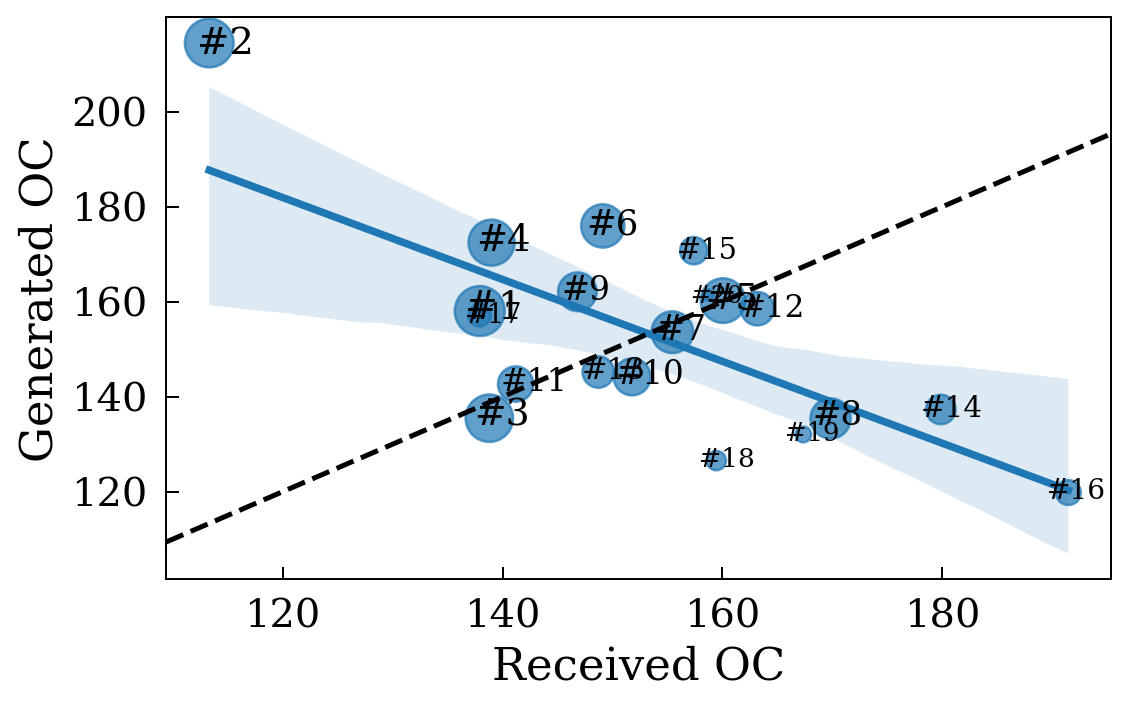
\includegraphics[width=0.8\linewidth,]{imagenes/Mean_rival_OC_vs_team_norm_efftime} 

}

\caption{Generated vs. received Offside Control. The values correspond to the average accumulated OC per effective time unit. The size of the nodes (and their labels) correlates with the ranking corresponding to all the matches analysed. The dashed line corresponds to $y=x$. The linear regression is shown in blue and has the equation $y = -0.86x + 285.42$, with $R^2 = 0.48$ and $RMSE = 14.96$. Teams above the dashed line have accumulated more Offside Controls than their rivals.}\label{fig:ranking}
\end{figure}

\begin{figure}[H]

{\centering 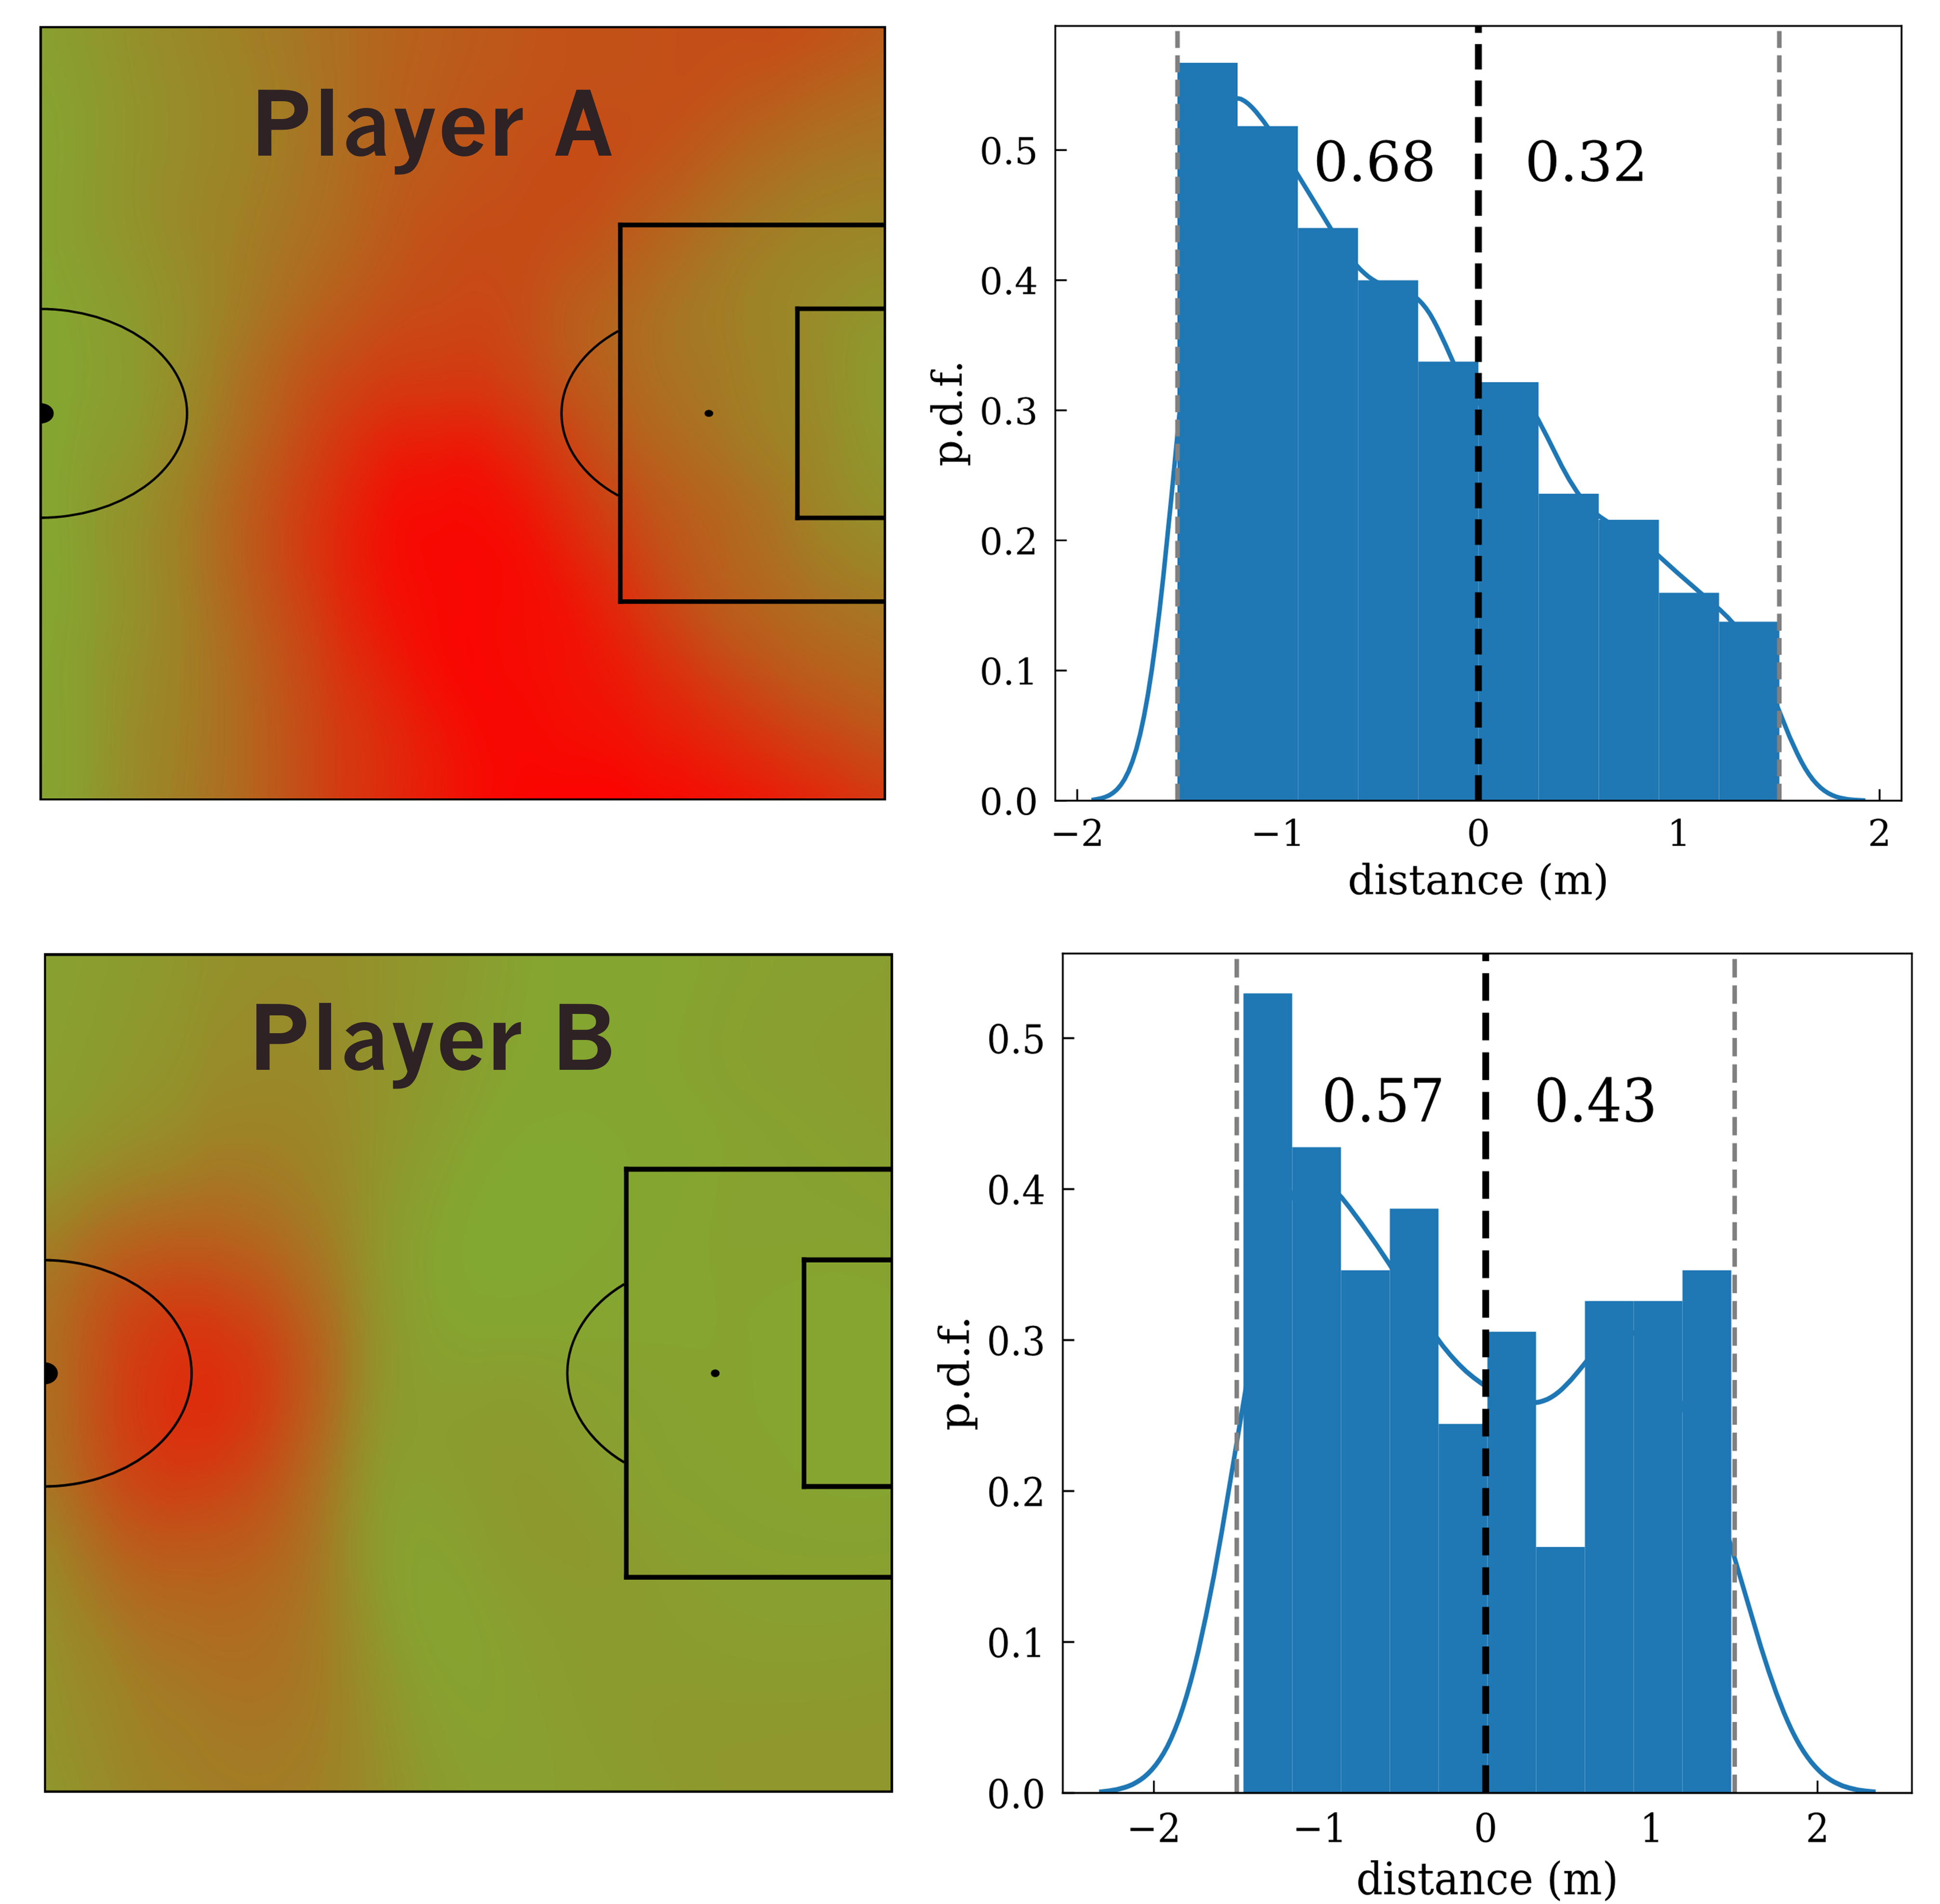
\includegraphics[width=0.7\linewidth,]{imagenes/forwards_OC} 

}

\caption{Effective Offside Control (EOC) of two different strikers, A (upper plots) and B (lower plots). On the left, the positions on the pitch where the two players generate EOC. On the right, the probability distribution function of the time spent at a distance from the offside line. Negative values indicate that the player is in the correct position, while positive values indicate that the player is offside. The EOC is normalised to the time played. The values on the right plot indicate the proportion of time a player is in front of or behind the offside line.}\label{fig:forwards}
\end{figure}

In this work, the Offside Control of a total of 442 players was characterized. With all this data, we calculated the percentage of time that strikers spend close to the offside line and what percentage of that time the striker is in a valid position. We call this percentage a player's Offside Time Efficiency Ratio (OTER). Next, we relate the OTER to the percentage of OC that is effective, i.e.~\(EOC/IOC\), and we call this percentage the \emph{Offside Control Efficiency Ratio (OCER)}. In Fig. \ref{fig:forwardsglob} (A) we show the relationship between OTER and OCER for the \(50\)\footnote{To ensure the statistical validity of the results, the study only included players who played at least 6 games.} forwards. We have obtained a positive correlation between the two metrics, as indicated by the solid blue line. This suggests that the more time a striker spends in a valid position near the offside line, the higher the probability of generating effective Offside Control.
However, the correlation coefficient between the two variables is low (\(R^2=0.2325\)), indicating that their relationship is complex and suggesting the effects of alternative variables not considered in our analysis. Finally, Fig. \ref{fig:forwardsglob} (B) shows the probability distribution function of the values of the OCER. We can see that most of the Offside Control generated by the strikers is effective, indicated by a probability distribution mainly above \(0.5\) and a mean of \(\langle OTER \rangle=0.7506\).

\begin{figure}[H]

{\centering 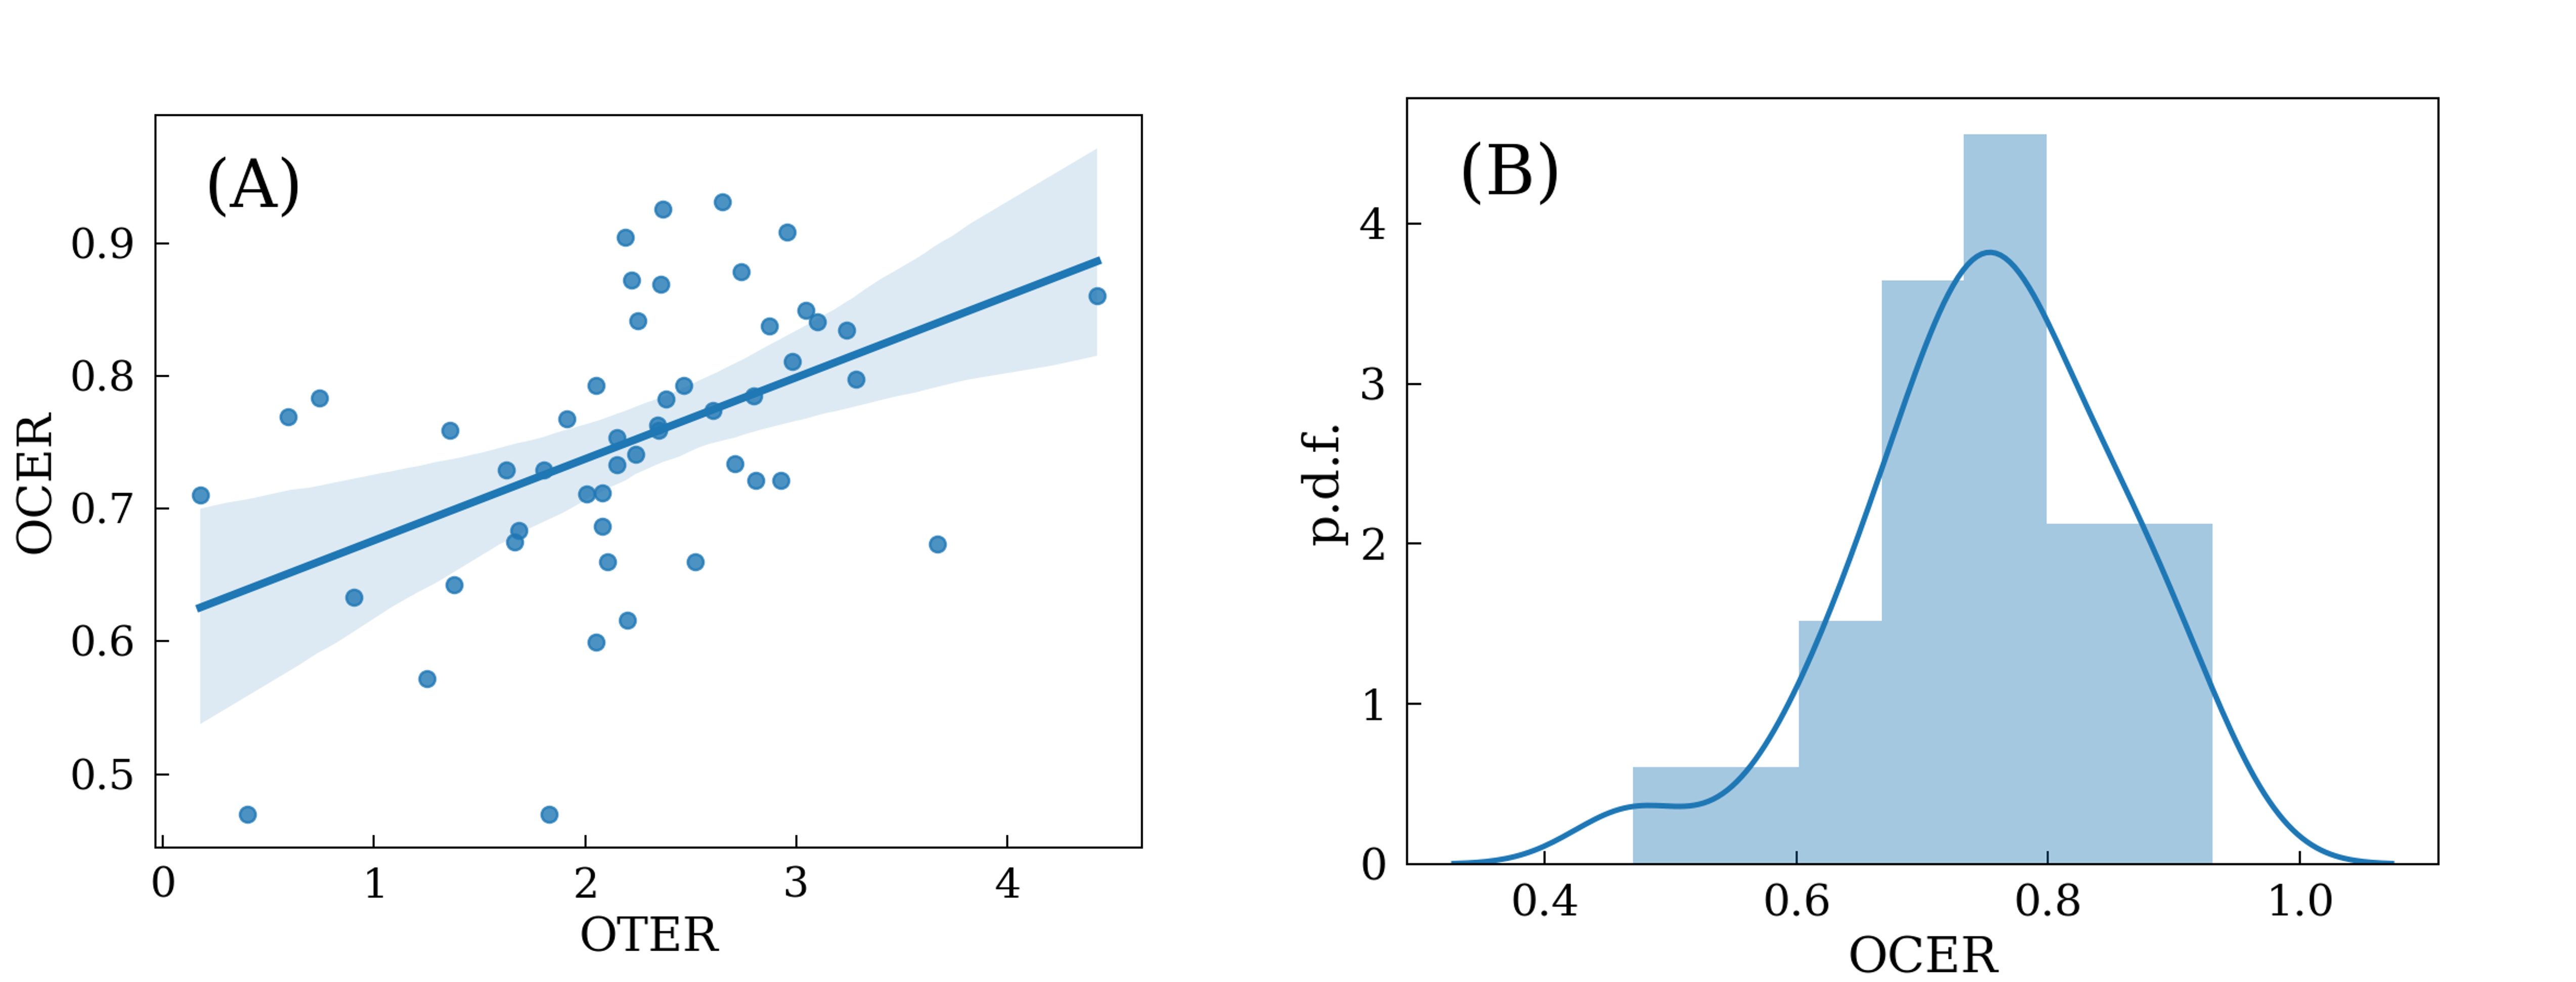
\includegraphics[width=0.8\linewidth,]{imagenes/av_eff} 

}

\caption{Interplay between Offside Time Efficiency Ratio (OTER) and Offside Control Efficiency Ratio (OCER). On the right, we show the OCER vs. OTER of the strikers.}\label{fig:forwardsglob}
\end{figure}

  \bibliography{bibliografia.bib}

\end{document}
